% !TEX root = main.tex
\chapter{System Overview}\label{cha:systemOverview}
This chapter provides the reader with a brief overview of the collimation system used in the \abbrLHC at \abbrCERN as well as a more detailed description of the rotational stage, which is the device in focus in this thesis. It also gives a short description of the piezoelectric actuator and its nonlinear effects. At the end of this chapter the present control approach is described in detail, including modeling of the rotational stage, system identification and controller structure.

\section{Crystal Collimators}
A collimator is a specially designed device, built to interfere with the beam and clean it from surrounding halo particles. To be able to meet the future demand of higher energy levels, a more efficient collimator is being developed at CERN. This new collimator, named goniometer, will utilize a crystalline solid to extract particles from the beam. A very simplified illustration of the crystal collimation principle is shown in Figure~\ref{fig:collimation}.

\begin{figure}[h!]
  \centering %crop: left bottom right top
  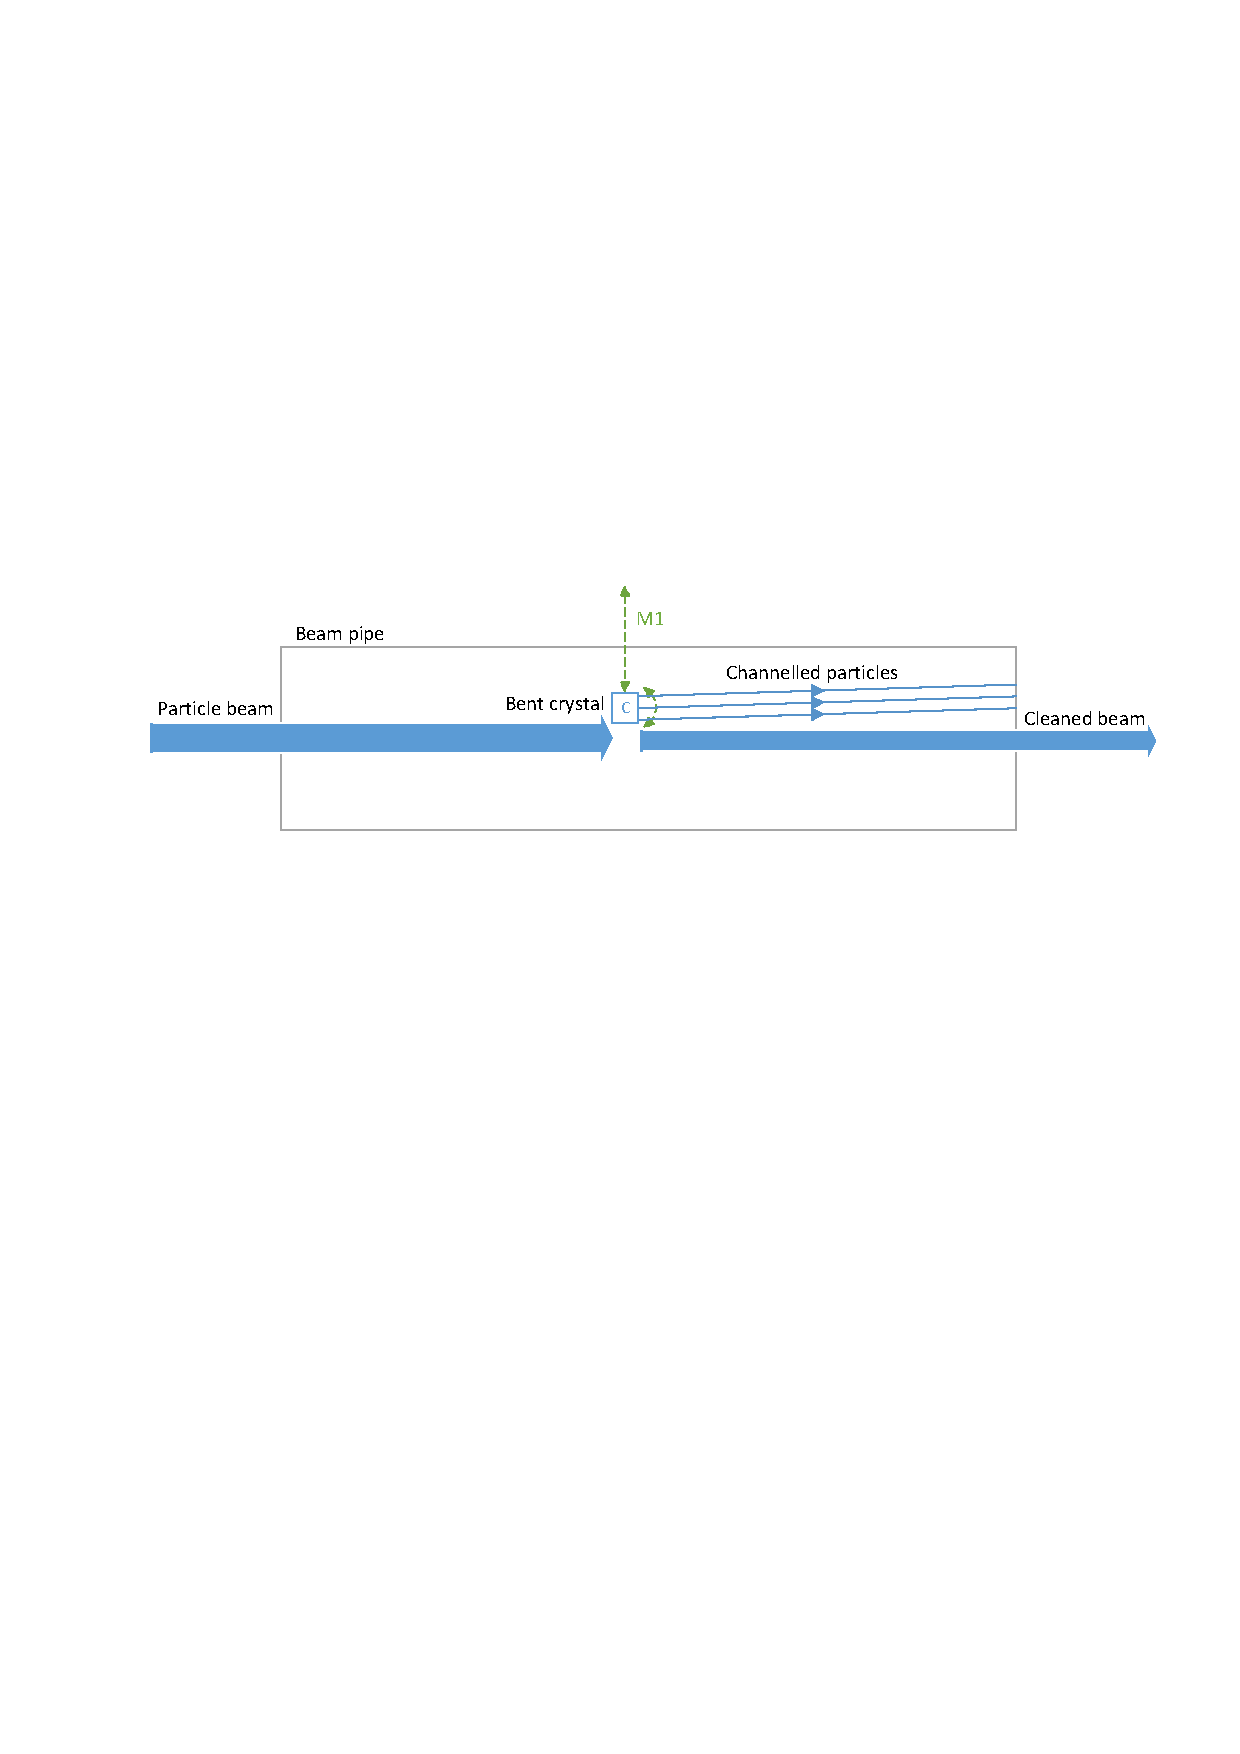
\includegraphics[width=1\textwidth, trim= 2cm 15.5cm 1cm 10cm, clip=true]{fig/matlab/collimation}
  \caption{\label{fig:collimation}Illustration of the crystal collimation principle as seen from above (top view in Figure~\ref{fig:collimator}). The dashed lines represent the linear and the rotational stage movement.}
\end{figure}

The block named "C" in Figure~\ref{fig:collimation} represents the bent crystal which can be moved into the beam by the linear stage and rotated by the rotational stage which is attached to the linear axis. The crystal's linear and rotational movement are indicated in the figure as green dashed lines. During operation, physicists will drive the crystal close to the beam, enter it with an angle and rotate it slightly (in the range of \unit{1}{\milli\rad}) until the channeling effect is detected. Channeled particles (illustrated as arrowed lines in Figure~\ref{fig:collimation}) will then bend off from the beam core to be absorbed further down the beam pipe.

The goniometer unit consists of a T-shape structure containing two linear and one rotational stage, as partly illustrated in Figure~\ref{fig:goniometer}.

\begin{figure}[h]
  \centering %crop: left bottom right top
  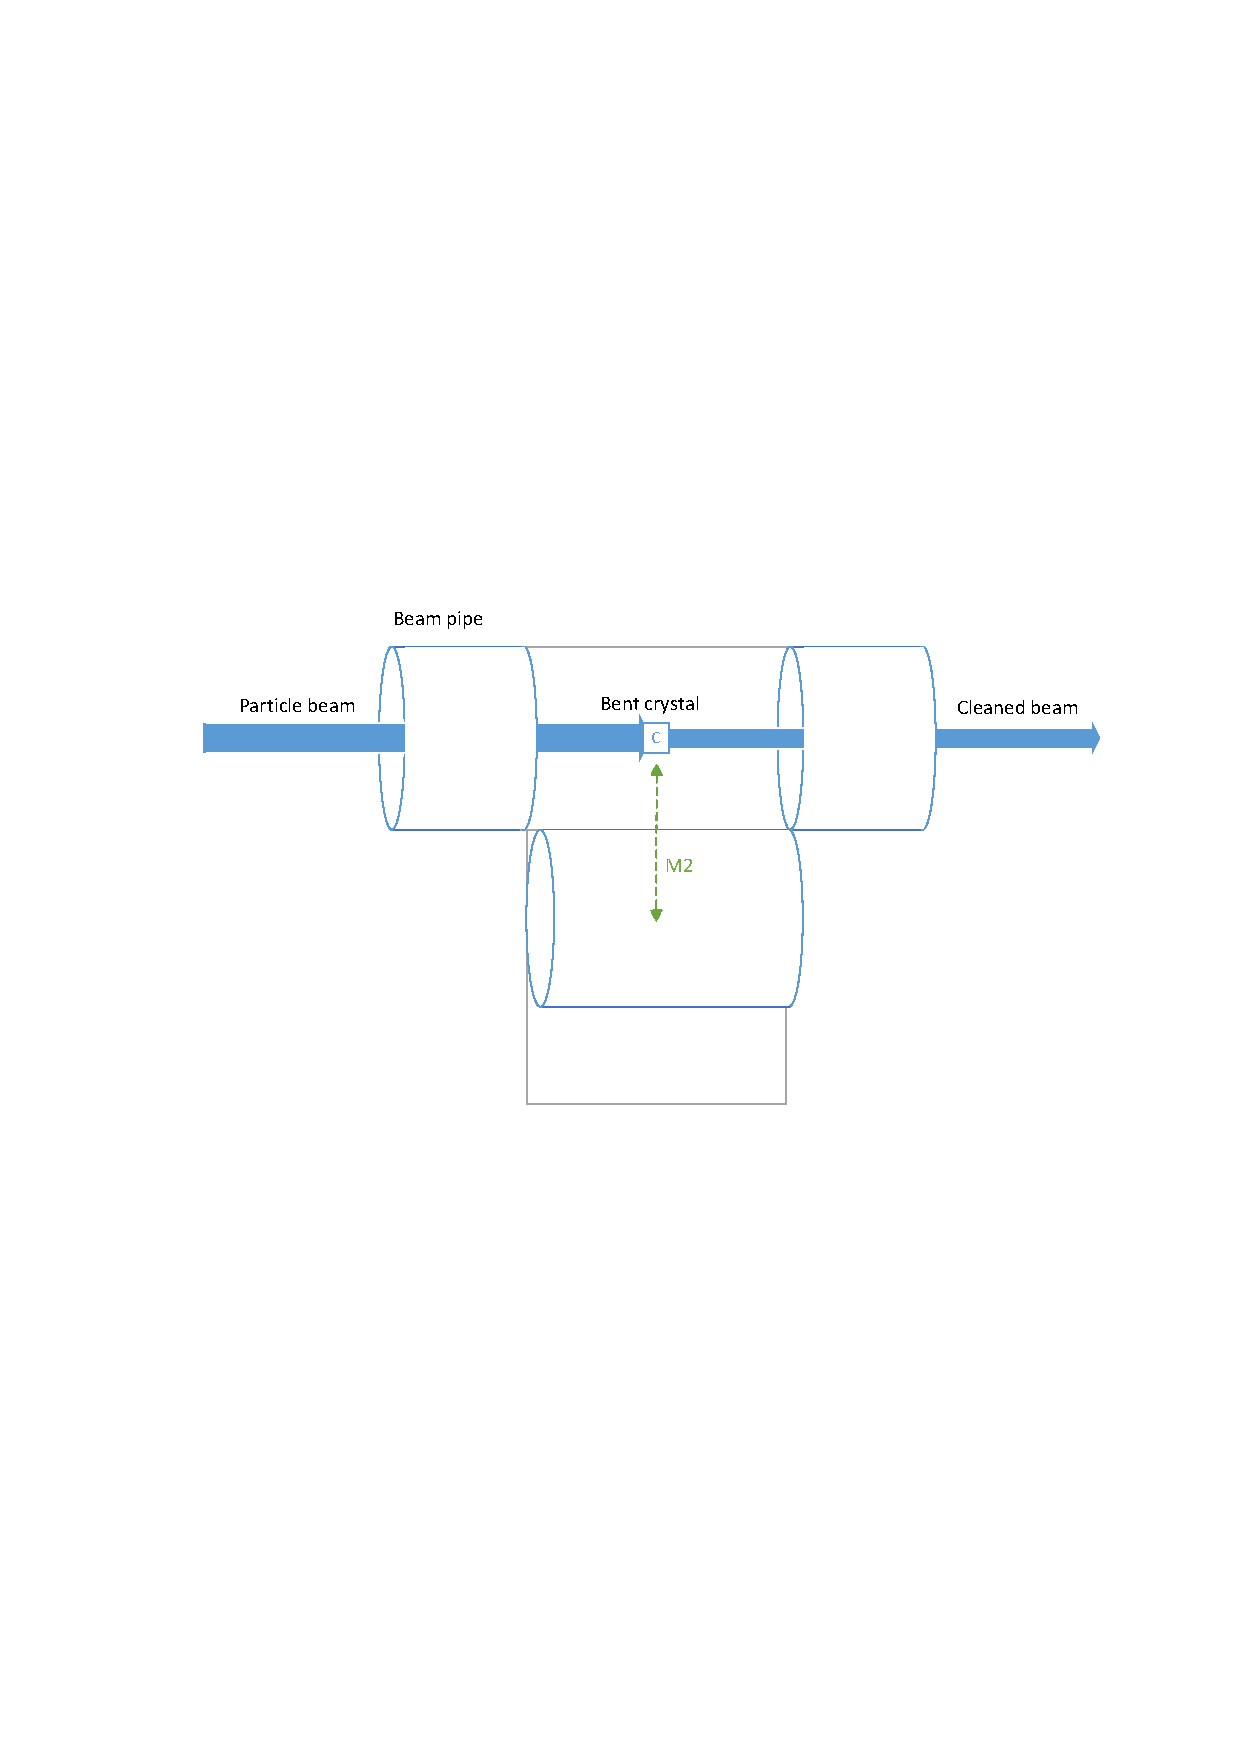
\includegraphics[width=1\textwidth, trim= 2cm 12cm 1cm 10cm, clip=true]{fig/matlab/goniometer}
  \caption{\label{fig:goniometer}Illustration of the crystal collimation principle as seen from the side (side view in Figure~\ref{fig:collimator}). The green dashed line represents the movement of the beam pipe piece.}
\end{figure}

Each linear stage is driven by a stepping motor, labeled as \emph{M1} in Figure~\ref{fig:collimation} and \emph{M2} in Figure~\ref{fig:goniometer}, separately controlled in open-loop by an individual drive unit. The motor driving the vertical axis, \emph{M2}, is used to move a piece of beam pipe inside the T-shape, giving access to the crystal to enter and to close it when the collimation system is out of operation. This movement is illustrated in Figure~\ref{fig:goniometer} with a green dashed line.

Figure~\ref{fig:collimator} shows the new goniometer. In the top view the rotational and the linear horizontal stage is indicated with labels. In this figure, the rotational stage is in its outer position. During operation it will be moved forward by the linear axis into the beam pipe. Figure~\ref{fig:collimator-through} shows the inside of the beam pipe during movement of the beam pipe piece, the same movement that Figure~\ref{fig:goniometer} is illustrating. In Figure~\ref{fig:collimator-mirror} the crystal support has been injected into the beam pipe. Note that the crystal itself is in this picture replaced by a small circular mirror.

\begin{figure}[tpb]
  \centering %crop: left bottom right top
  \subfloat[][\label{fig:collimator-side}Side view]{
  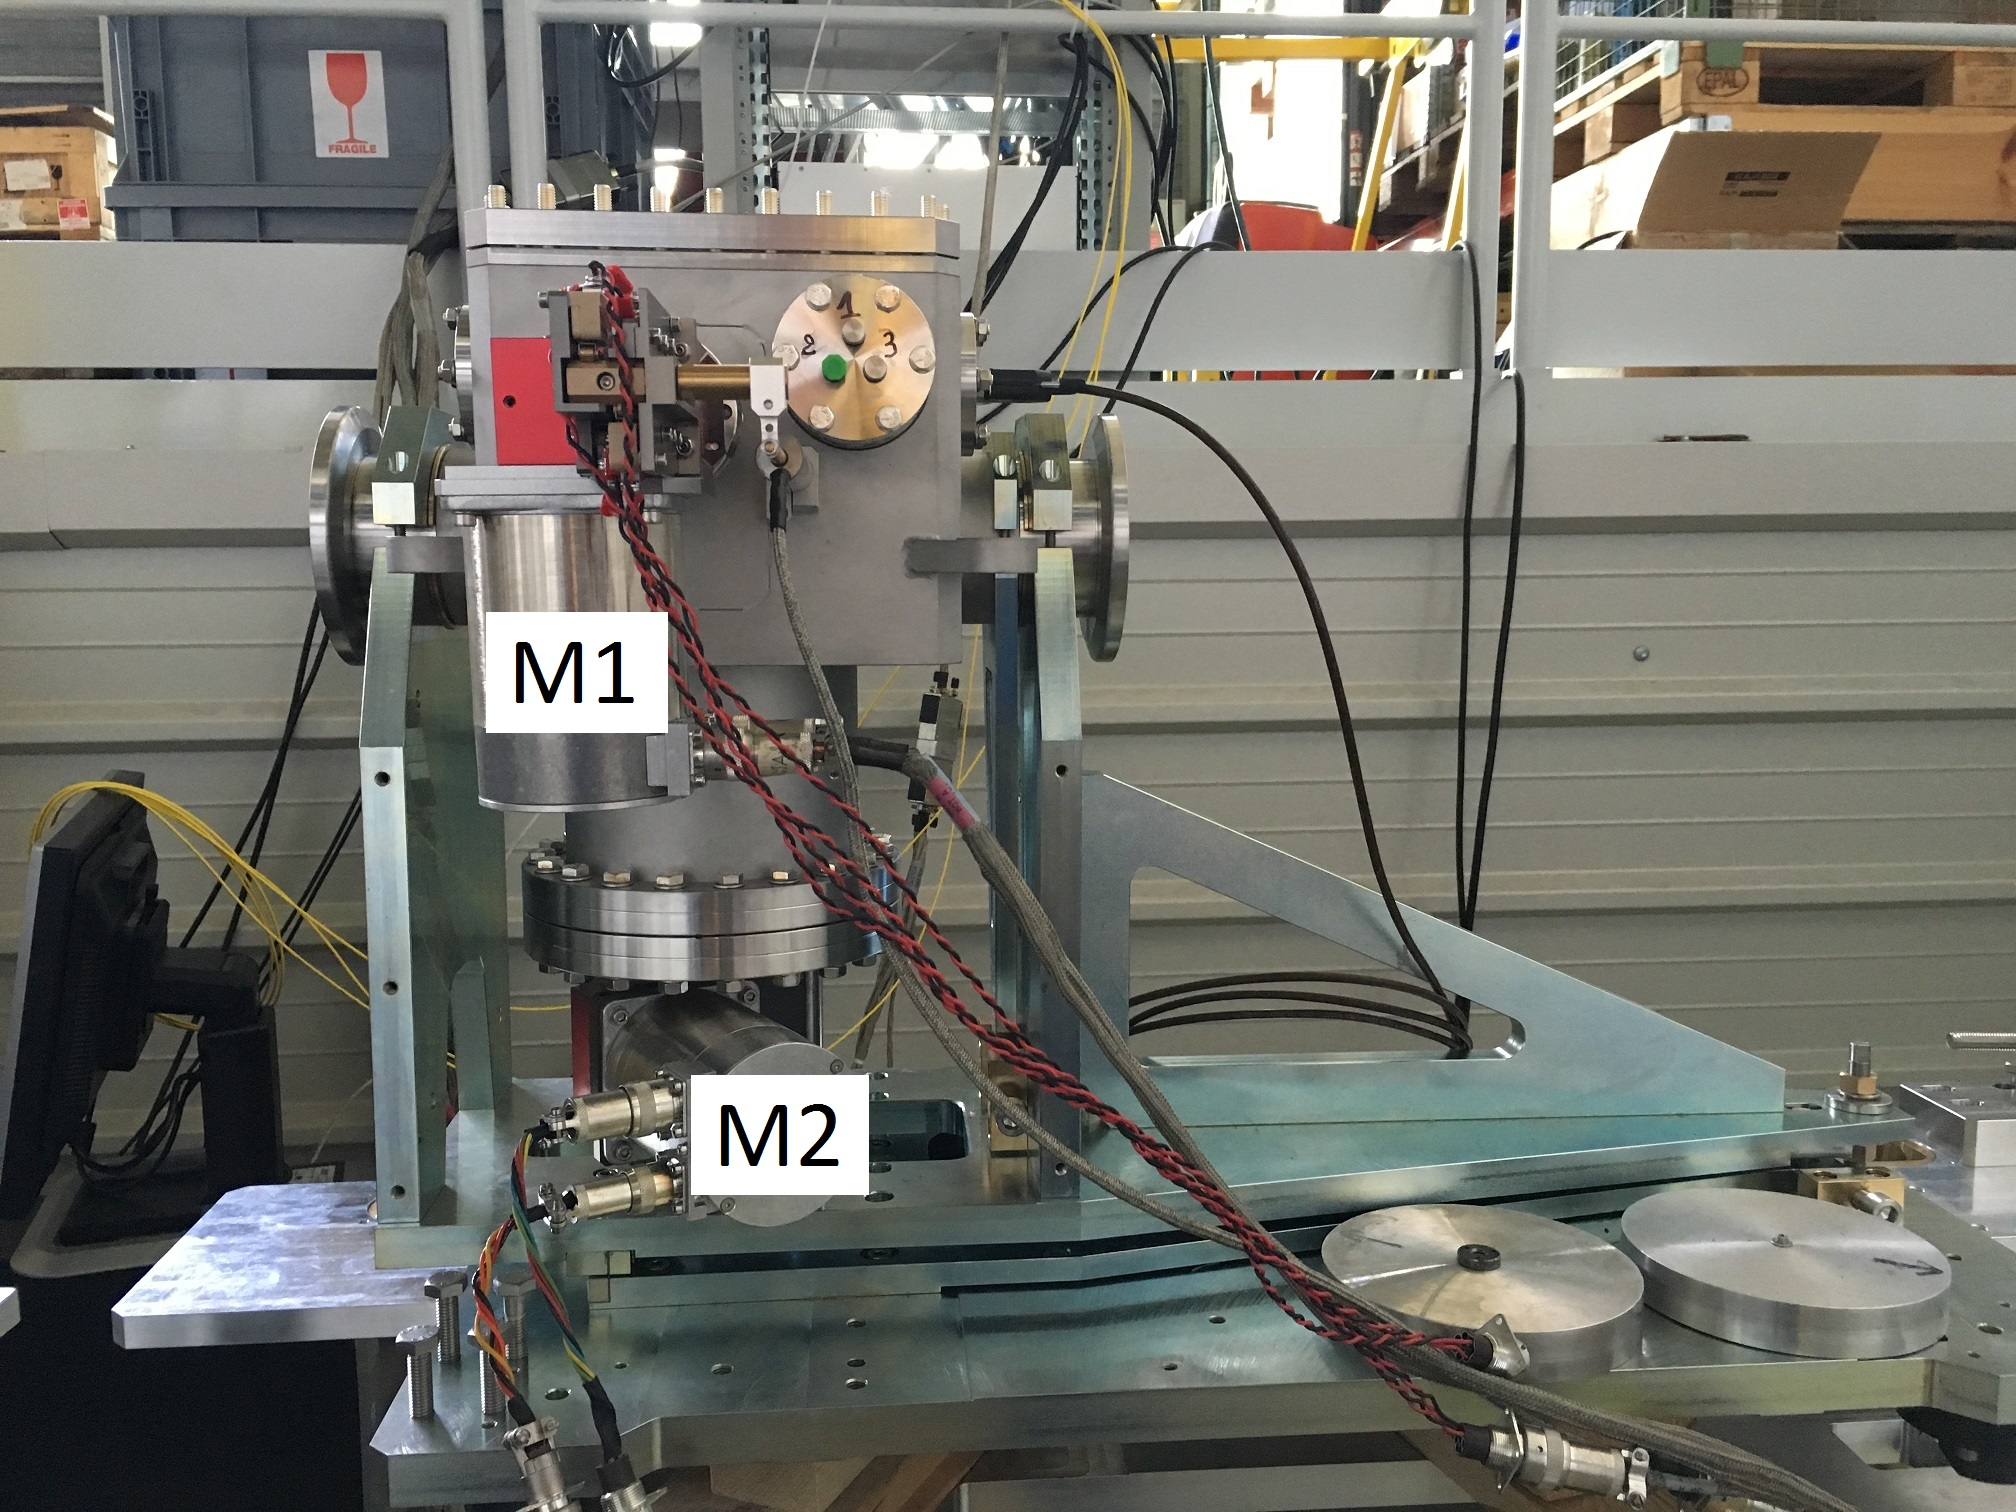
\includegraphics[width=0.5\textwidth, trim=2cm 11cm 2cm 5cm, clip=true]{fig/collimator-side}}
  \qquad
  \subfloat[][\label{fig:collimator-top}Top view]{
  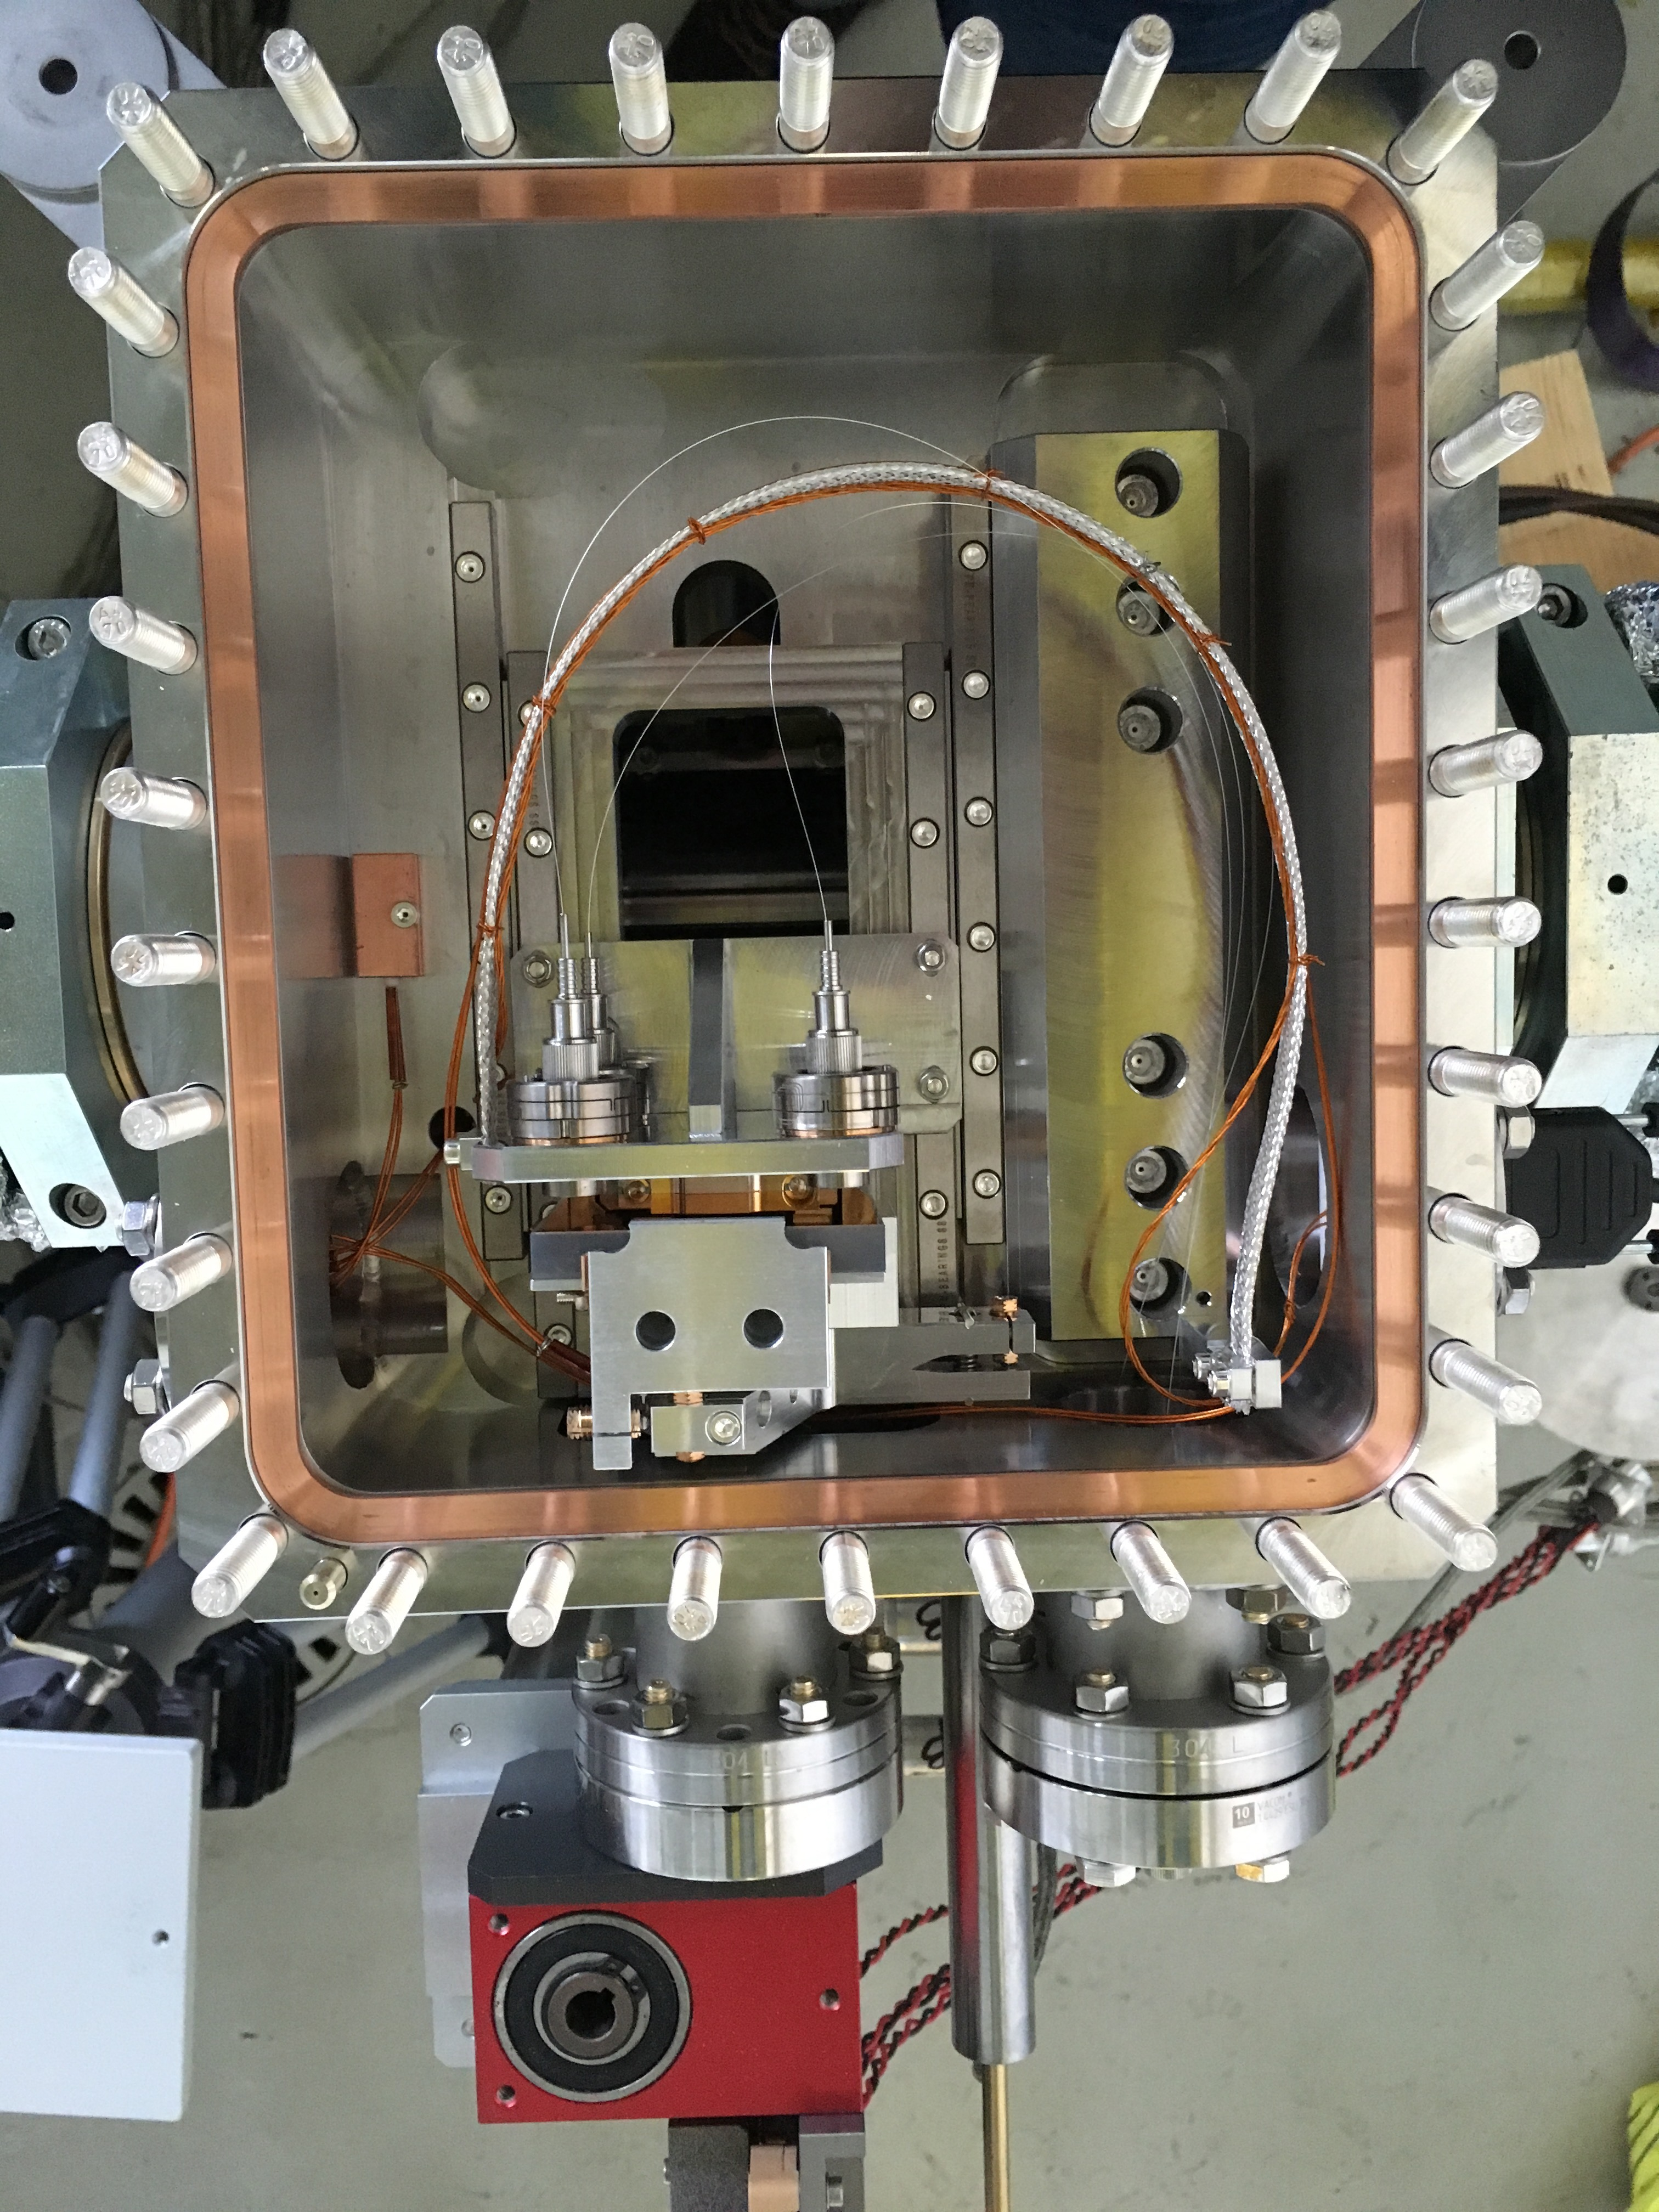
\includegraphics[width=0.42\textwidth, trim=0cm 0cm 0cm 0cm, clip=true]{fig/collimator-top}}
  \caption{\label{fig:collimator} The new goniometer from the side (a) and the top (b).}
\end{figure}

\begin{figure}[tpb]
  \centering %crop: left bottom right top
  \subfloat[][\label{fig:collimator-through} Giving access]{
  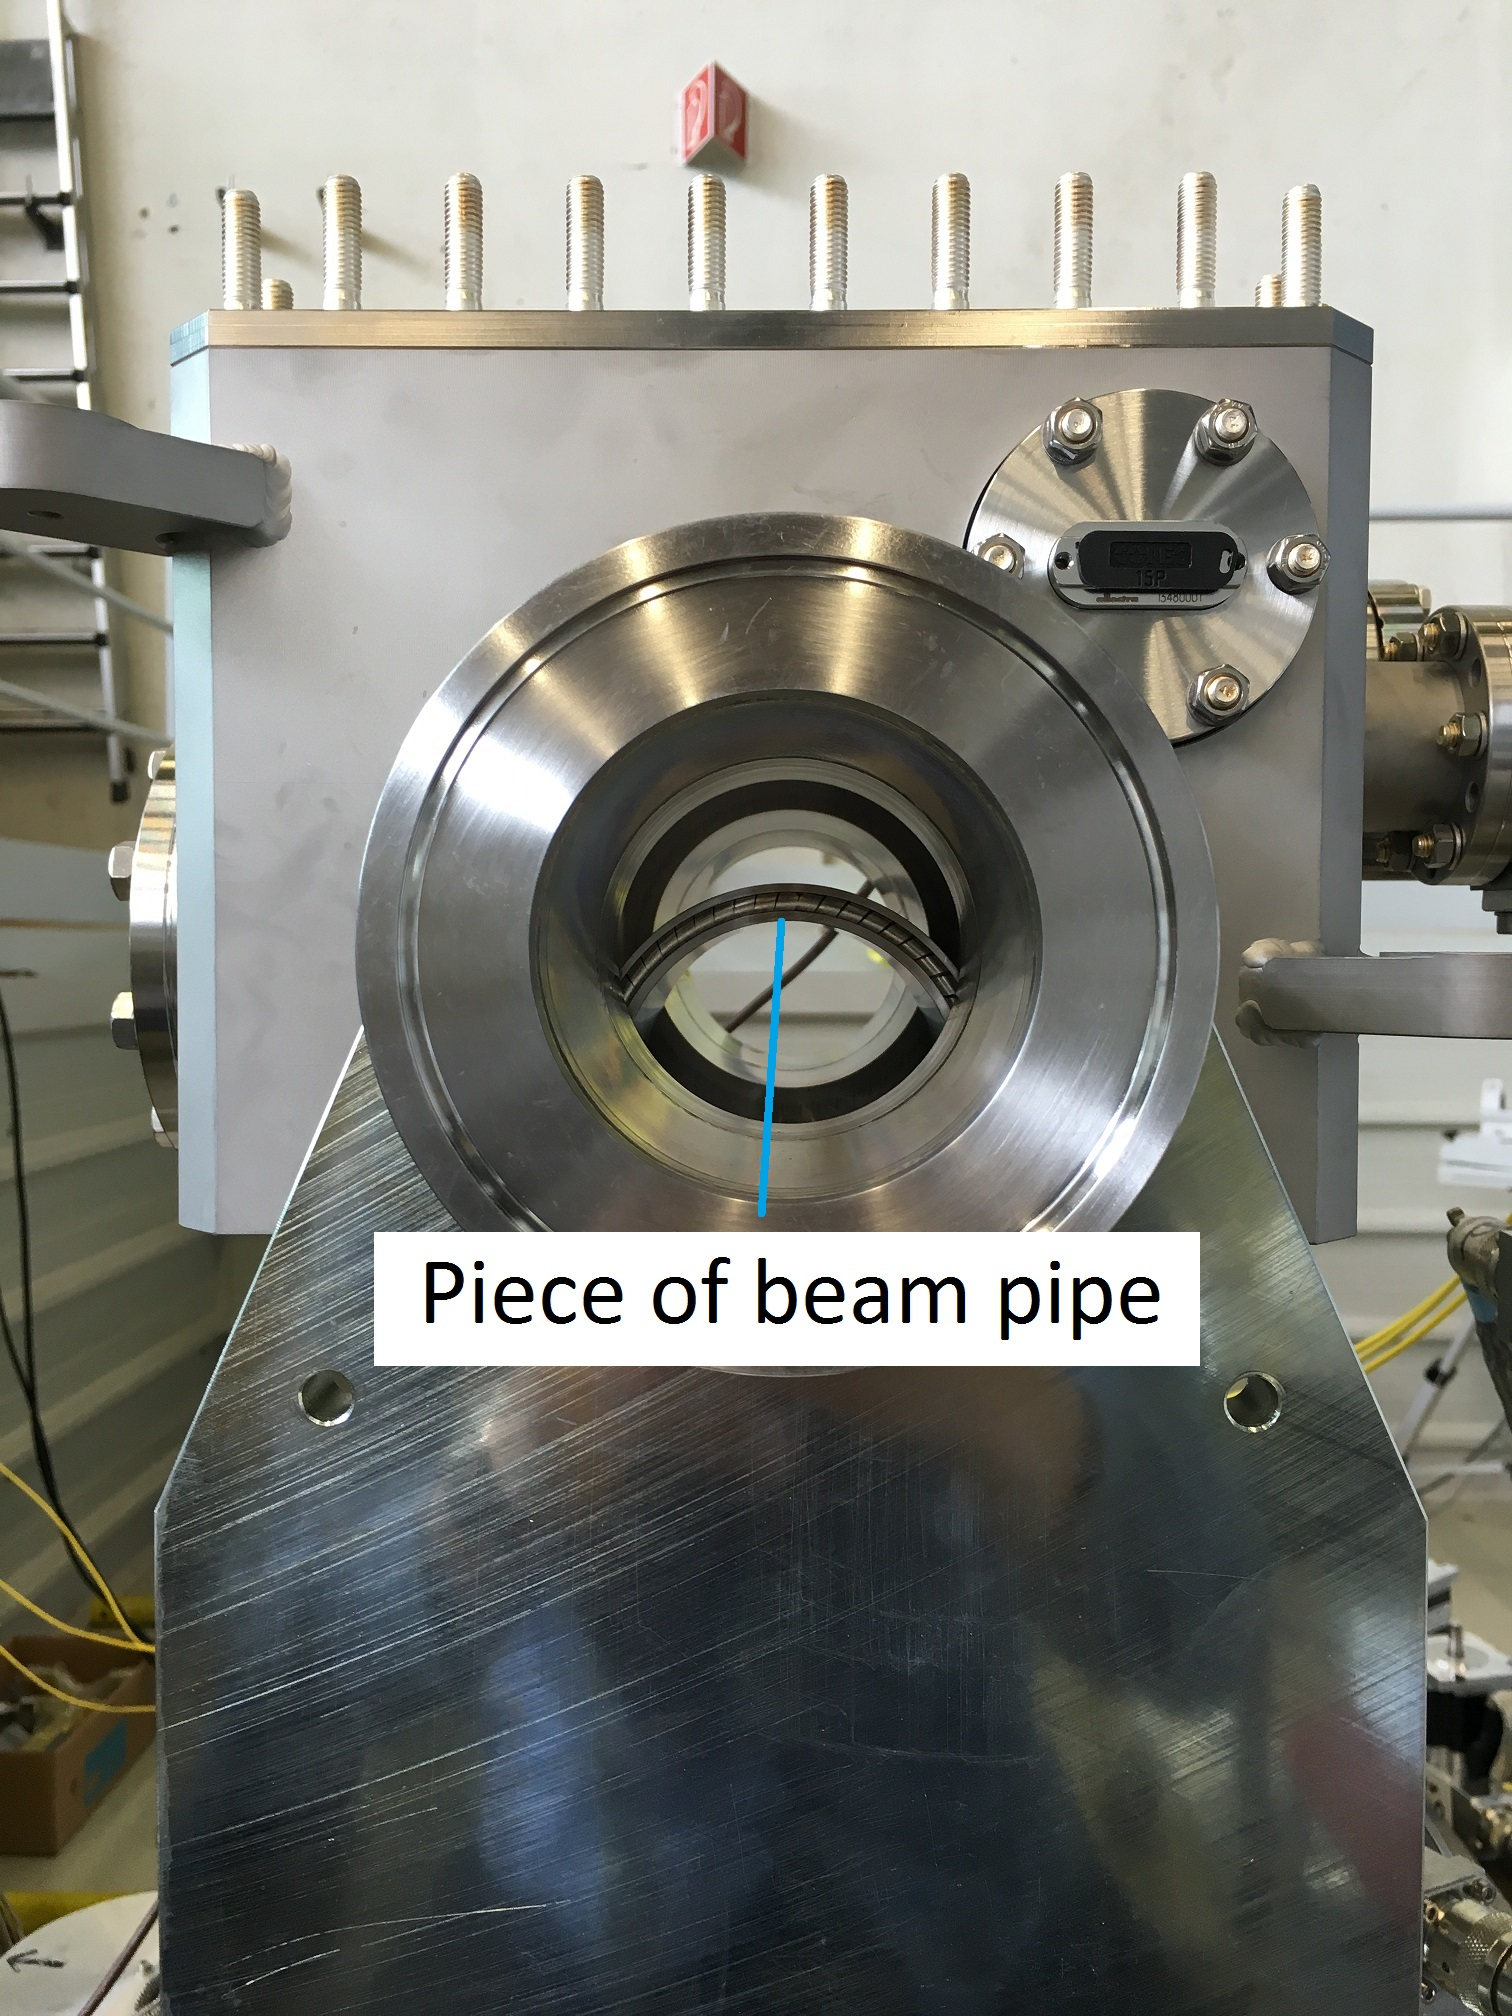
\includegraphics[width=0.42\textwidth, trim=3cm 12.8cm 2cm 5cm, clip=true]{fig/collimator-through}}
  \qquad
  \subfloat[][\label{fig:collimator-mirror} Insertion of crystal]{
  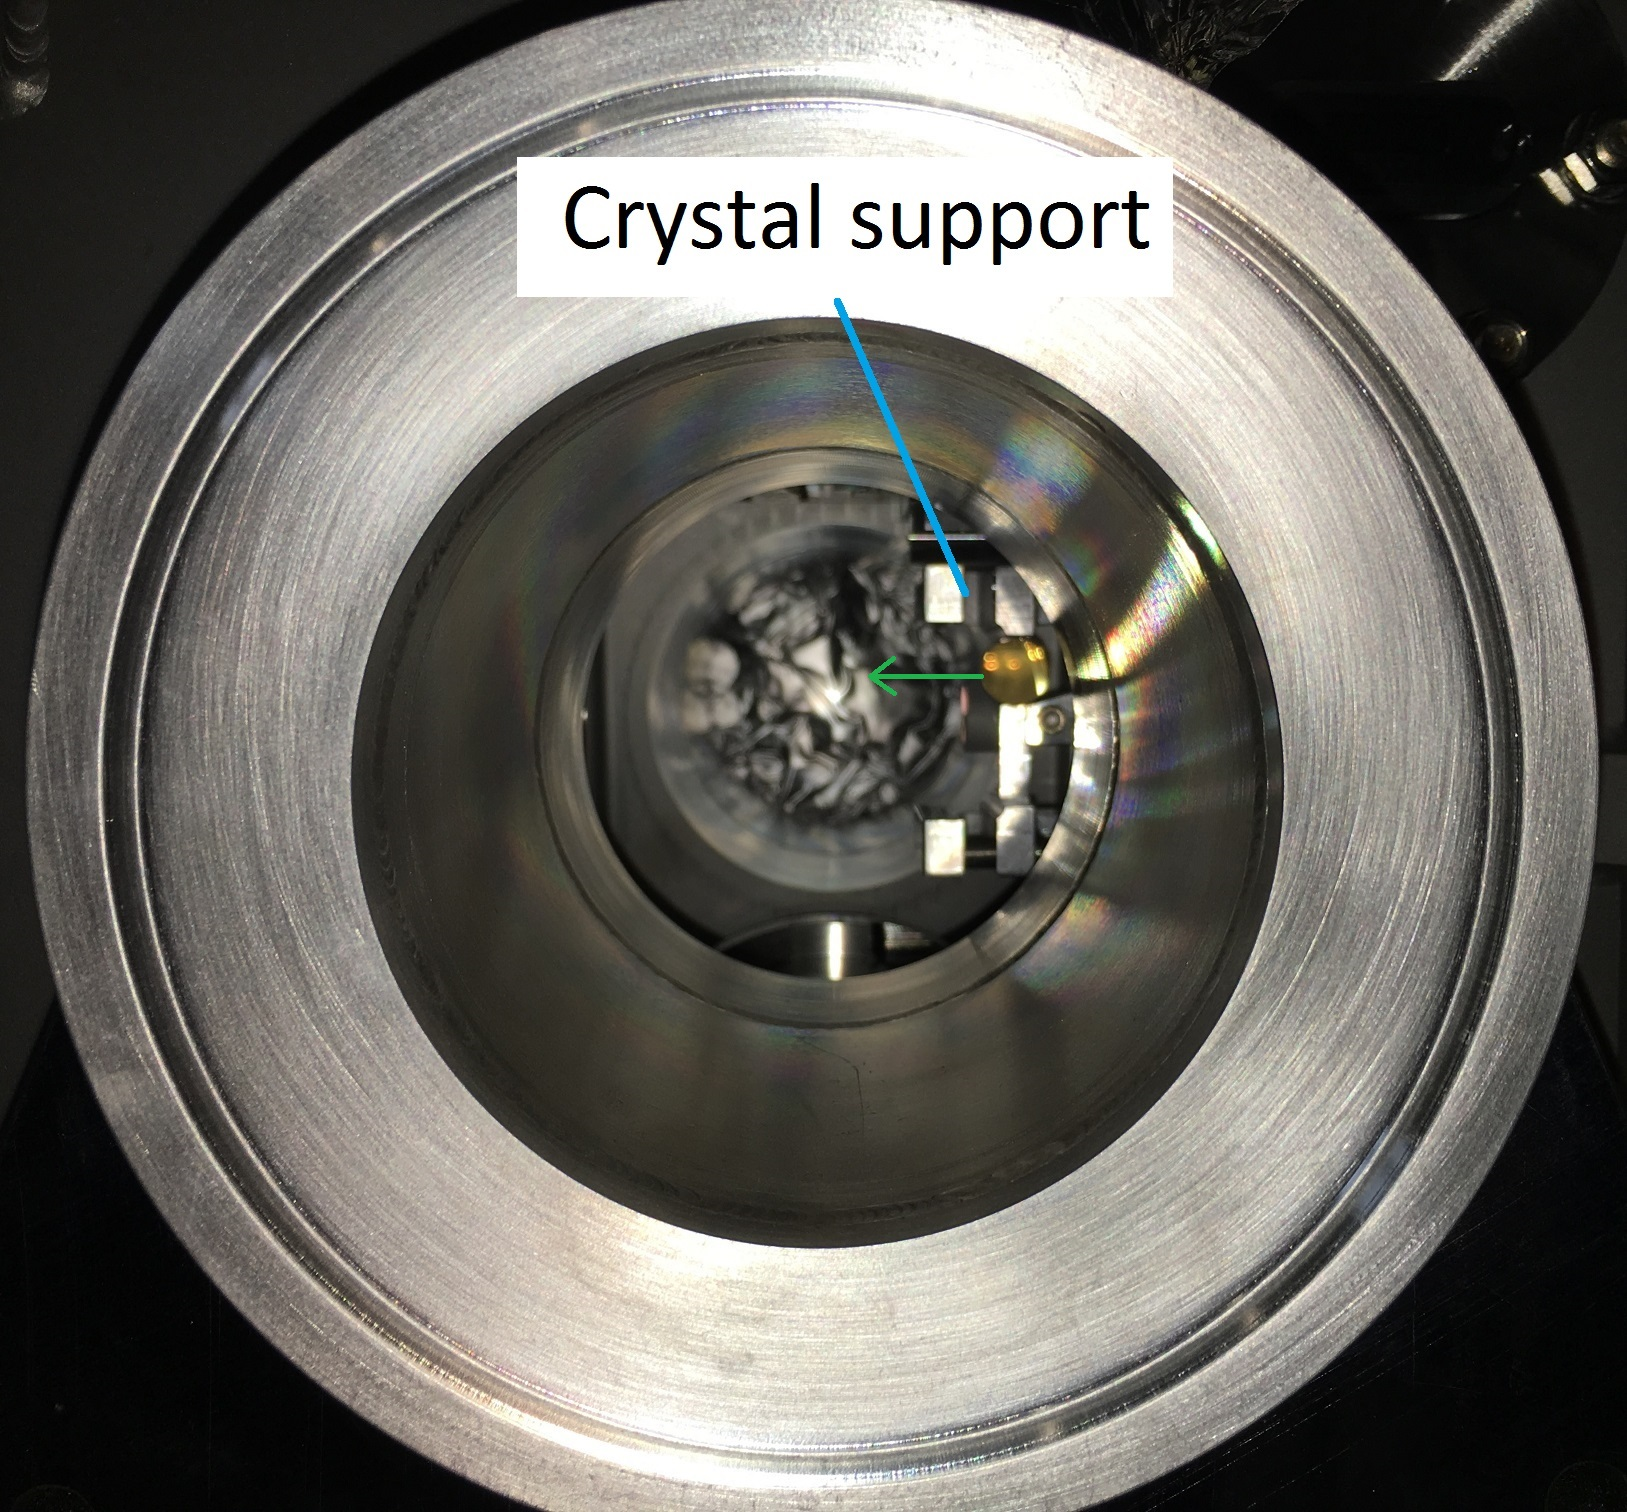
\includegraphics[width=0.5\textwidth, trim=0cm 0cm 0cm 0cm, clip=true]{fig/collimator-mirror}}
  \caption{\label{fig:collimator-t} The new goniometer with the beam pipe piece half-way out (a) and the crystal inserted into the beam pipe (b).}
\end{figure}

\FloatBarrier
\section{Rotational Stage}
\label{sec:rotational_stage}
The rotational stage as shown in Figure~\ref{fig:rotationalstage} is composed of a monolithic amplifying structure, a prestressed piezoelectric stack actuator and an interferometer measurement system. The flexure-hinge based structure, avoids sliding parts and thereby enhance precision by reducing the number of nonlinear effects (e.g. backlash and friction). A piezoelectric stack actuator is exploited to generate the rotational movement by interacting on a amplifying lever that applies the force on the rotational head a few millimeters from the center of rotation, marked as a white "X" in the picture. This amplifying structure gives the rotational stage a range of \unit{20}{\milli\rad} from a nominal linear range of \unit{30}{\micro\meter}.  The \abbrPEA is prestressed in order to enhance the overall stiffness as well as keeping the stack in place. This combination leads to a clear resonant structure, due to the characteristics of the \abbrPEA and the flexure structure, demanding a properly designed controller.

\begin{figure}[h!]
  \centering
  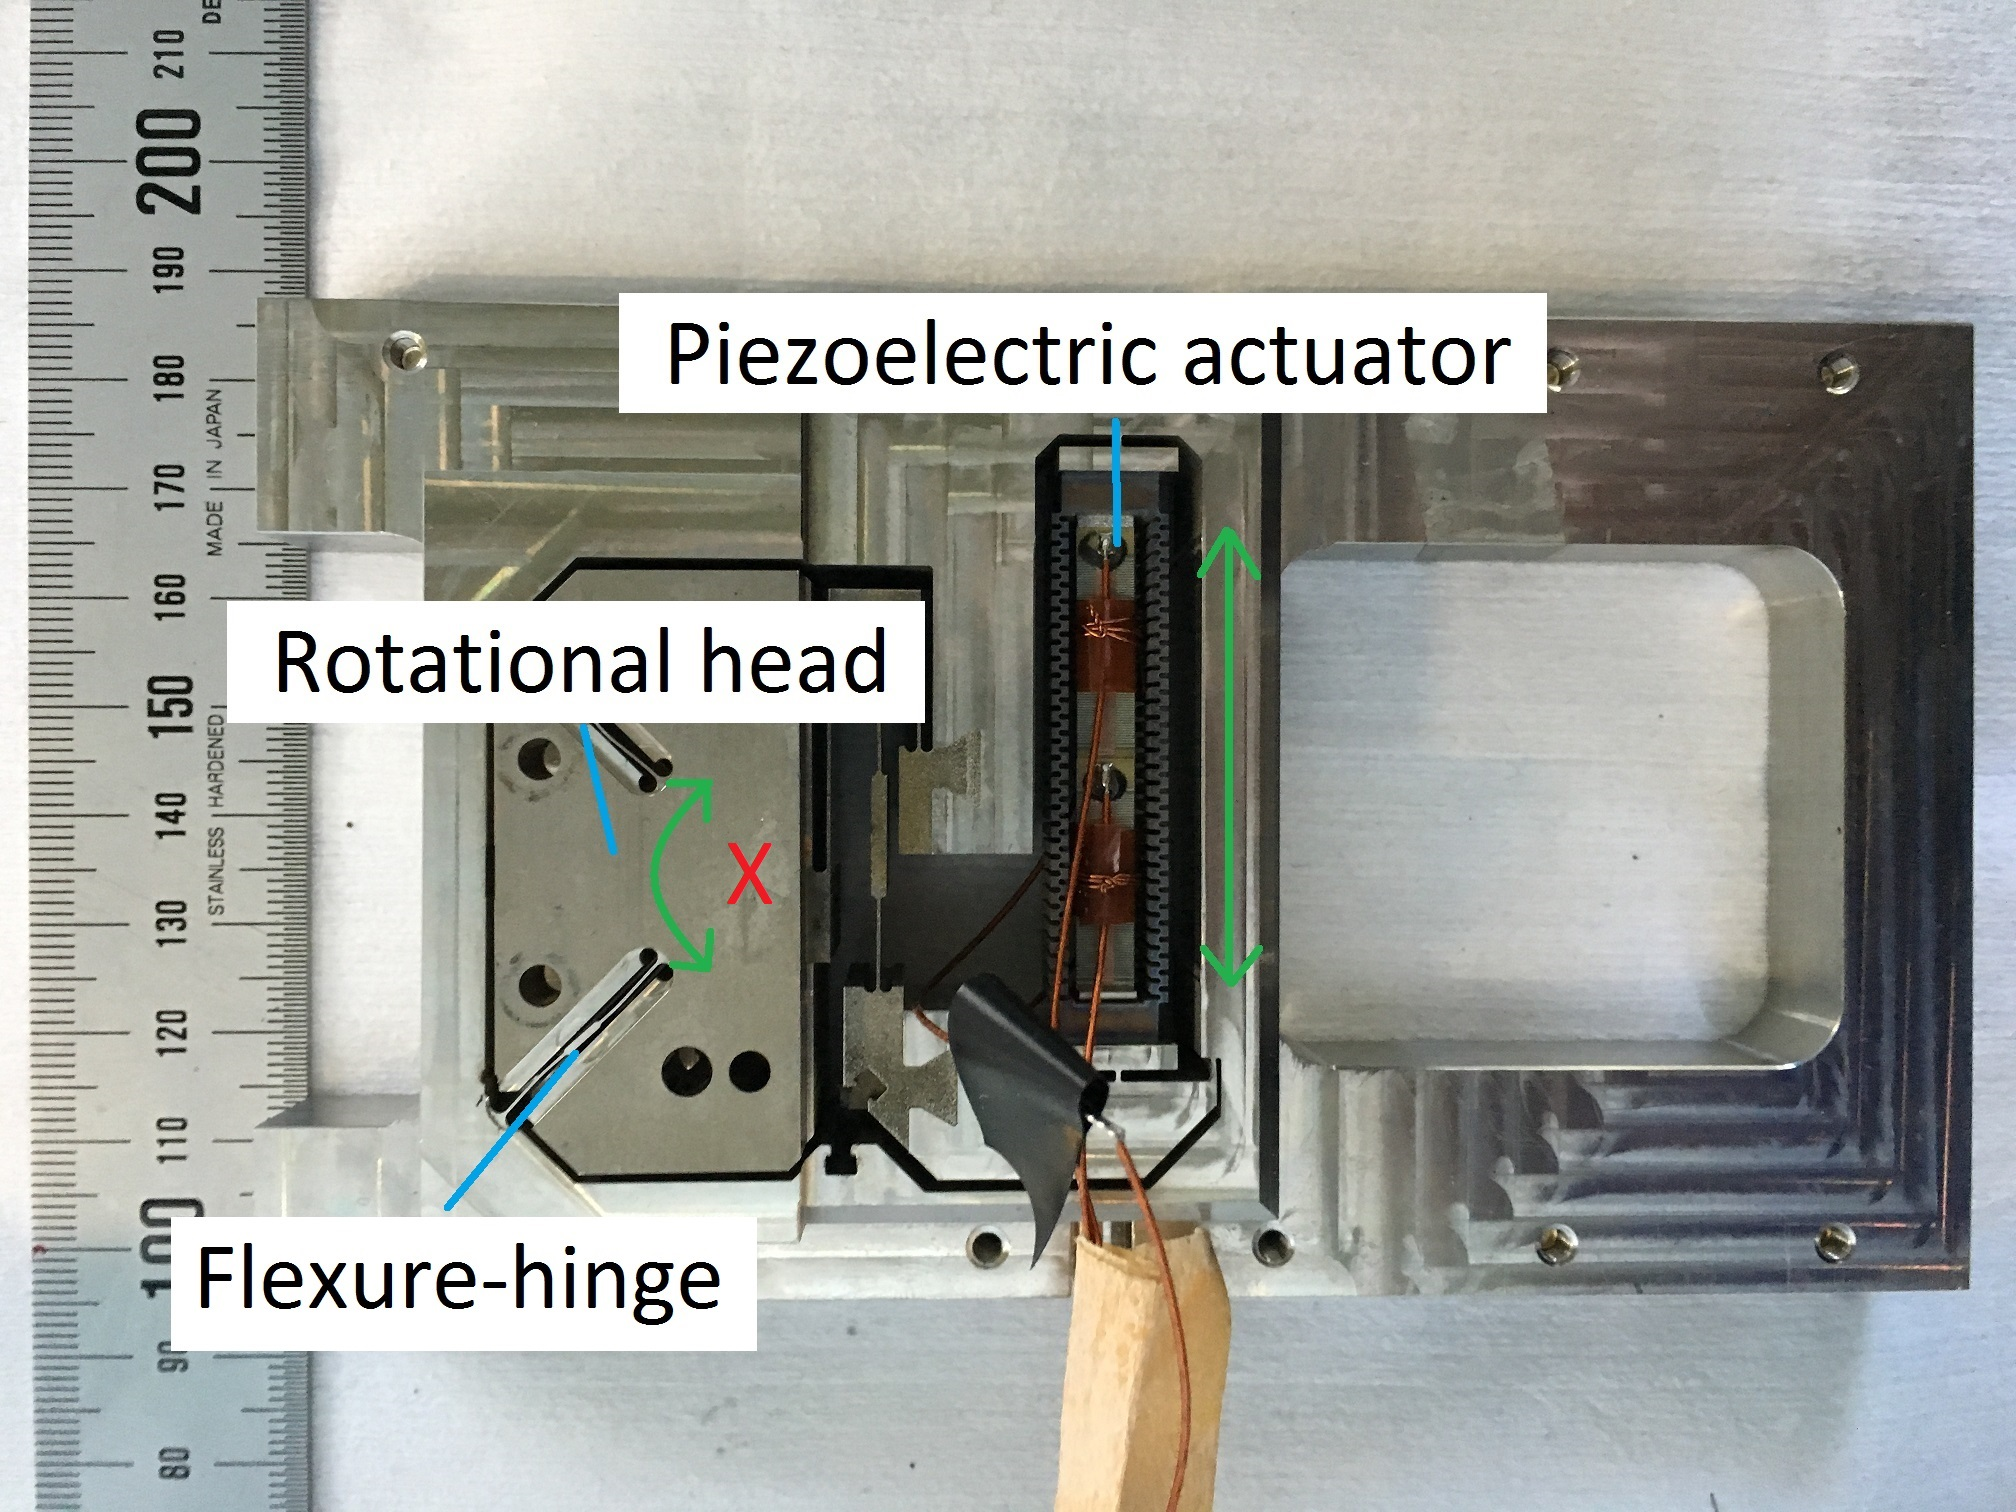
\includegraphics[width=0.7\textwidth]{fig/rotational-stage.jpg}
  \caption{\label{fig:rotationalstage} Piezo-actuated rotational stage used in the new goniometer.}
\end{figure}

For the measurement system, three interferometric heads are placed on top of the rotational stage as seen Figure~\ref{fig:rotationalstage-side}, pointing towards a mirror that is attached to the crystal support and to the rotational head, perpendicular to the plane of rotation. The setup allows for measurements of both the yaw, depicted in Figure~\ref{fig:rotationalstage}, and the roll angle (the coordinate system is defined with respect to the beam), but only the yaw angle is used in the feedback to the rotational stage control loop. Note that the crystal is mounted below the rotational head and that only the top of the crystal support is shown in the picture.

\begin{figure}[h!]
  \centering
  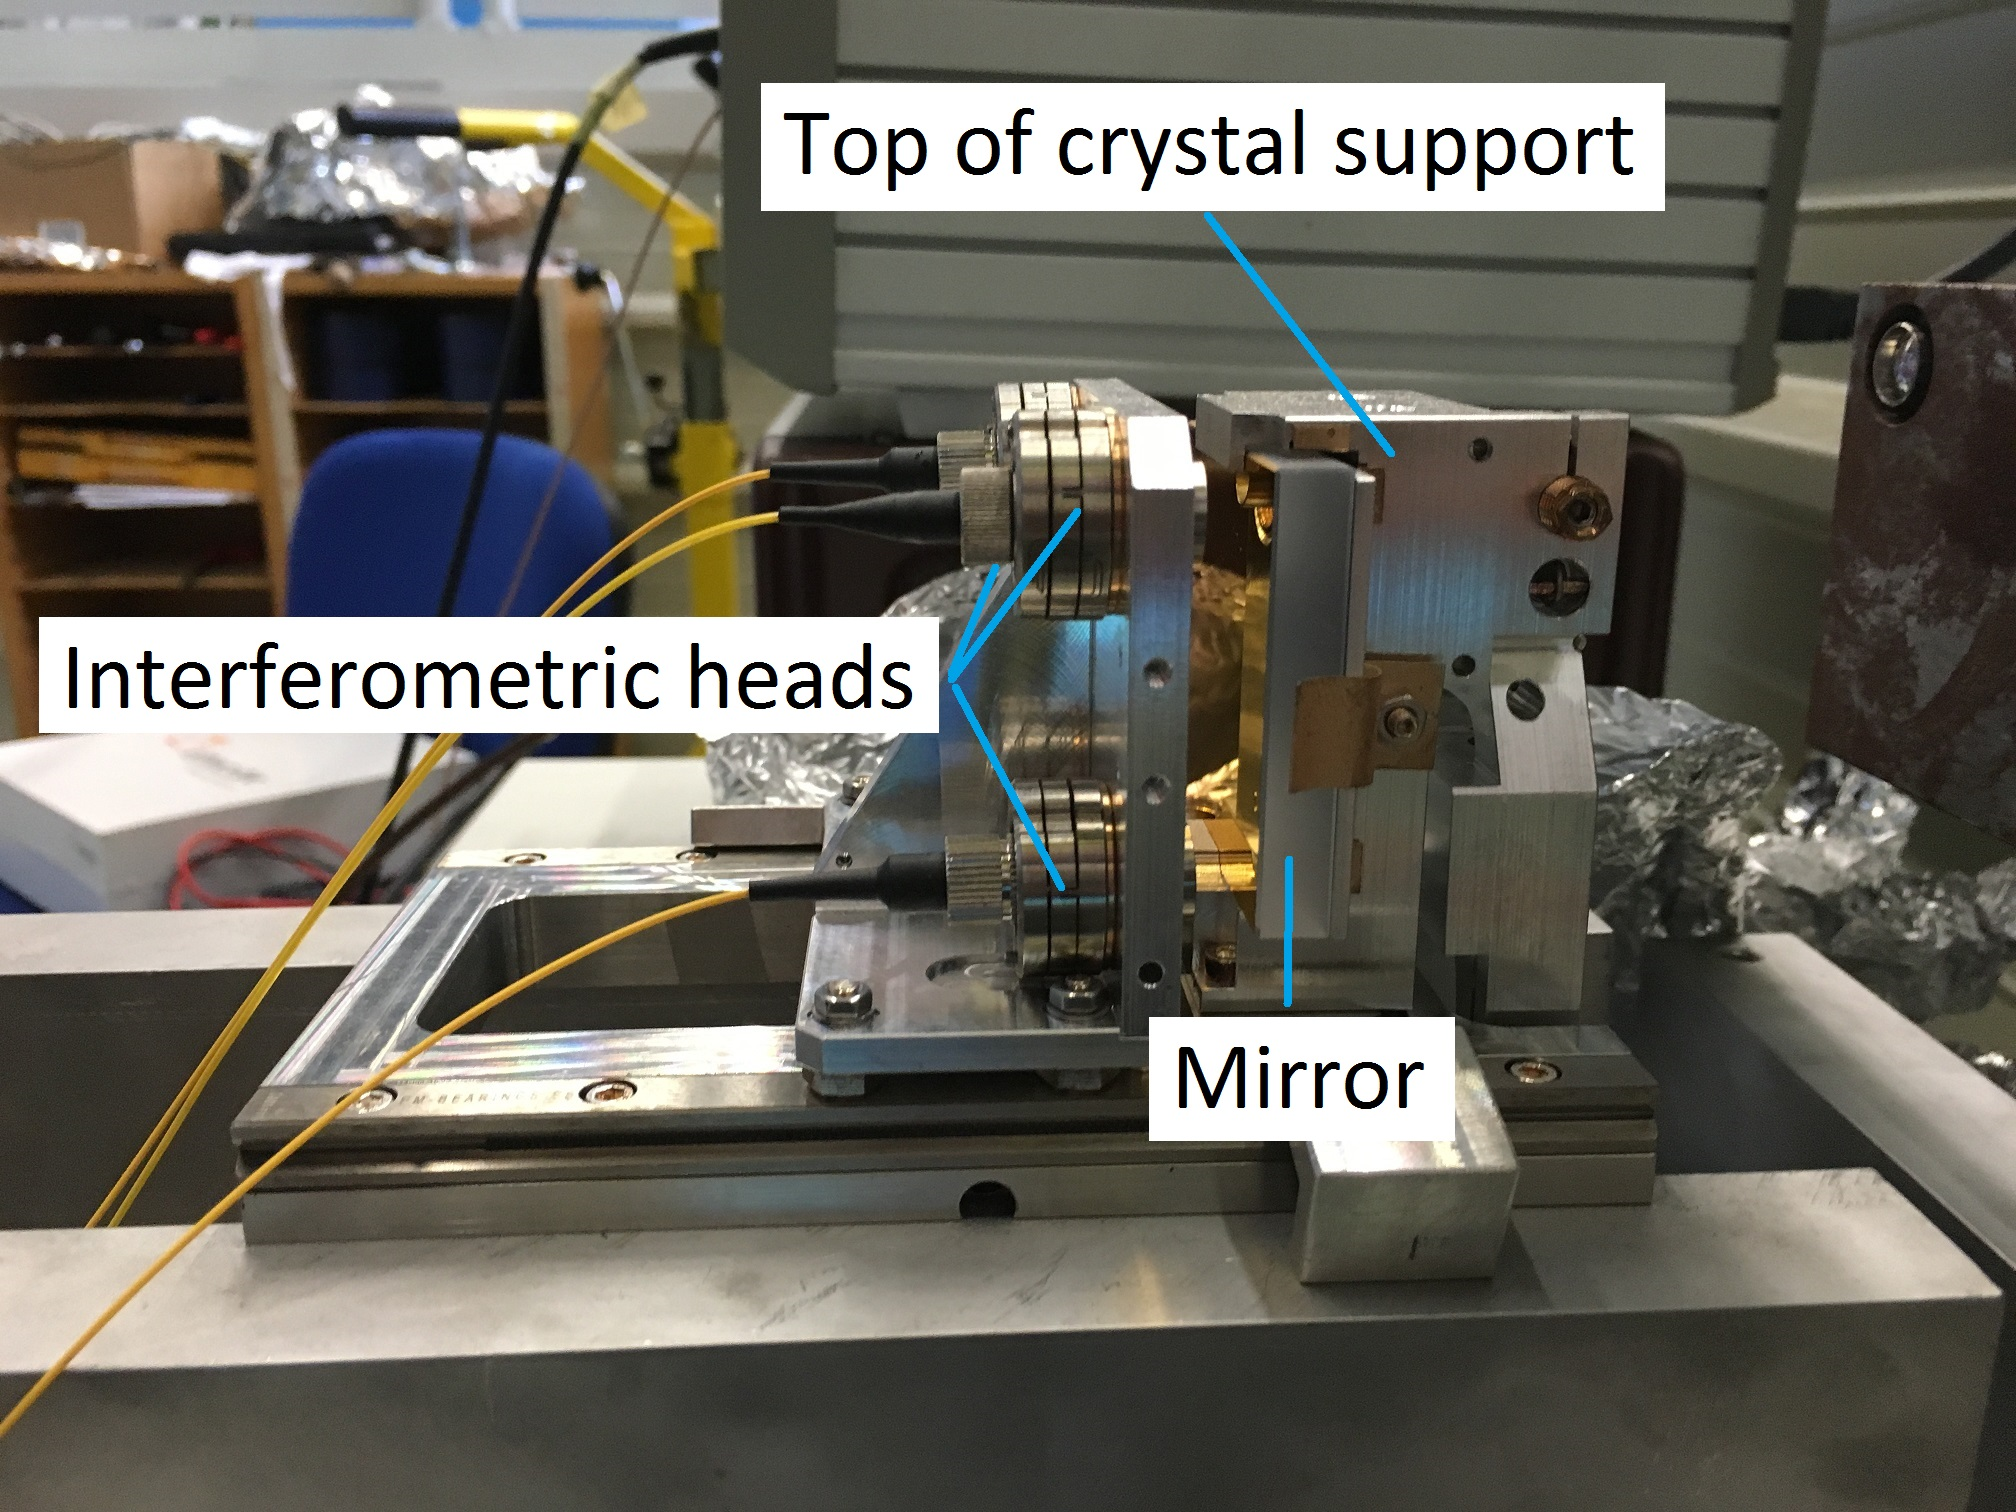
\includegraphics[width=0.7\textwidth]{fig/rotational-stage-interferometer.jpg}
  \caption{\label{fig:rotationalstage-side} Rotational stage with the crystal support and the interferometric system mounted on top.}
\end{figure}

\section{Piezoelectric Stack Actuators}
The rotational stage uses a linear piezoelectric stack actuator to create the movement. It provides a displacement range from 0 to \unit{30}{\micro\meter}, corresponding to -20 and +150 V, respectively. The actuators are made of many thin, stacked electro-active ceramic disks, electrically connected in parallel. This construction allows for a high stiffness actuator that still can exhibit long displacement ranges \citep{Piezo:2008}.

\subsection{Hysteresis Effect}
The hysteresis effect is a nonlinear effect that is present during the operation of piezoelectric actuators. It occurs when the driving direction is reversed and originates from the polarization and the molecular effects in the piezo-ceramic. It depends on the amplitude of the applied voltage but also on the frequency of the input signal \citep{Qingson:2016}. Figure~\ref{fig:hysteresis} illustrates the hysteresis effect. One can see how the same voltage, e.g. 60 V, corresponds to an angular position of \unit{5.2}{\micro\rad} in one direction and to \unit{7.2}{\micro\rad} in the opposite direction.

\subsection{Creep Effect}
The creep effect is another nonlinear effect that is present during the operation of piezoelectric actuators. The effect is a slow elongation or contraction of the actuator displacement over time with a constant driving signal and is caused by thermal effects in the piezo-ceramics. Figure~\ref{fig:creep} illustrates the creep effect. One can see how the rotational stage slightly drifts off from the reference after the applied negative step, increasing the tracking error over time.

\begin{figure}[h!]
  \centering %crop: left bottom right top
  \subfloat[][\label{fig:hysteresis} Hysteresis loop]{
  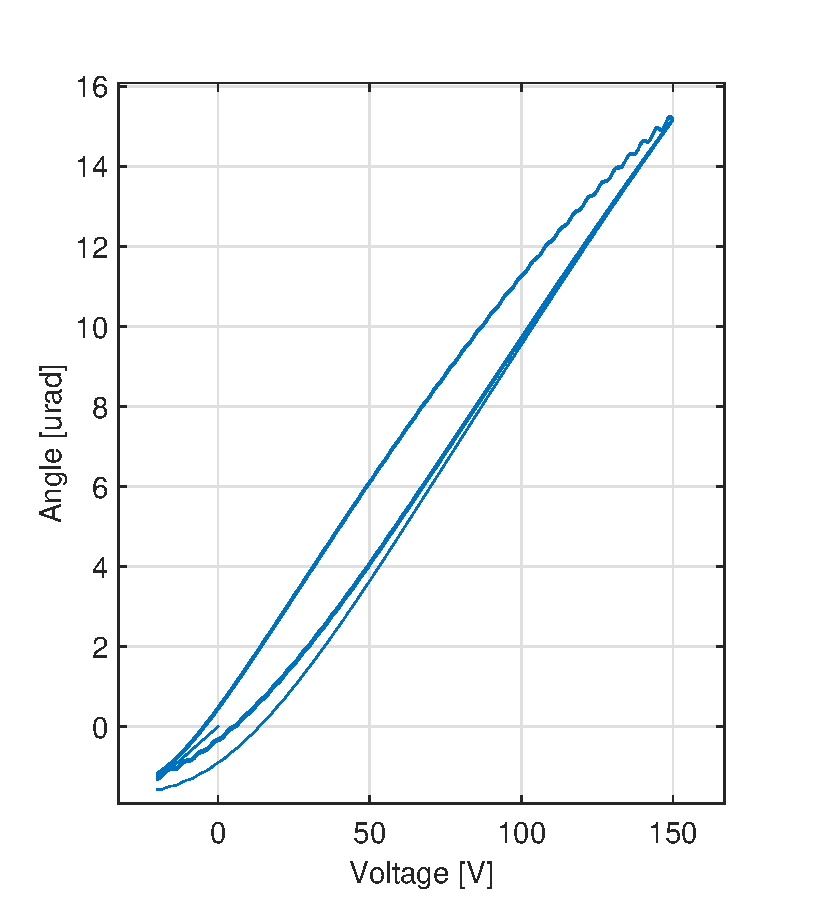
\includegraphics[width=0.46\textwidth, trim=0cm 0cm 1cm 0cm, clip=true]{fig/matlab/hysteresis.eps}}
  \qquad
  \subfloat[][\label{fig:creep} Creep effect]{
  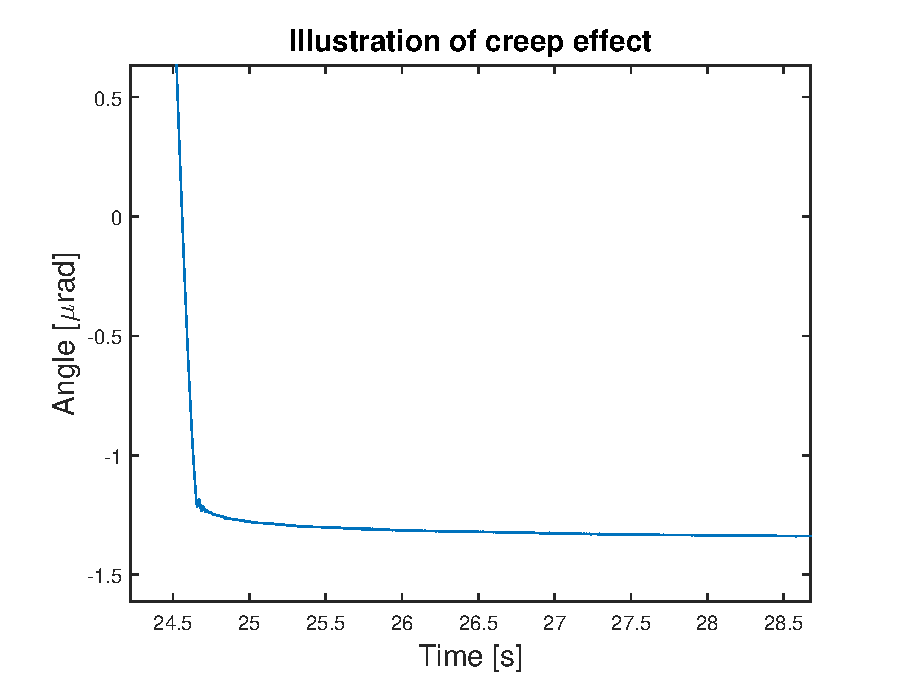
\includegraphics[width=0.46\textwidth, trim=0cm 0cm 1cm 0cm, clip=true]{fig/matlab/creep.eps}}
  \caption{\label{fig:effects} Illustration of the hysteresis effect (a) and creep effect (b). Note that the creep effect can last up to 10-15 minutes even if the plot only shows the development over 4 seconds.}
\end{figure}

The creep effect is in this project (and many others) efficiently suppressed by the feedback controller requiring no precise modeling and cancellation technique.

\section{Rotational Stage Modeling}
The piezo-actuated rotational stage is modeled by a Hammerstein structure, adop-ted by the authors in \citep{ButcherController:2015}, allowing them in principal, to decouple the nonlinear hysteresis from the linear system dynamics. The employed Hammerstein structure is depicted in Figure~\ref{fig:hammerstein} and consists of a \emph{Static Hysteresis} (rate independent) model and a \emph{Linear Dynamics} model. {\abbrPEA}s are known to show hysteretic behavior with a nonlocal memory (the current output does not only depend on the current input voltage but also on its history) as described in \citep{ButcherIdentification:2015}. This behavior is modeled by a generalized Maxwell-slip compensation model, described in \ref{sec:maxwell}. The extracted linear dynamics is identified using the described procedure in \ref{sec:linsys}.

\begin{figure}[h]
  \centering %crop: left bottom right top
  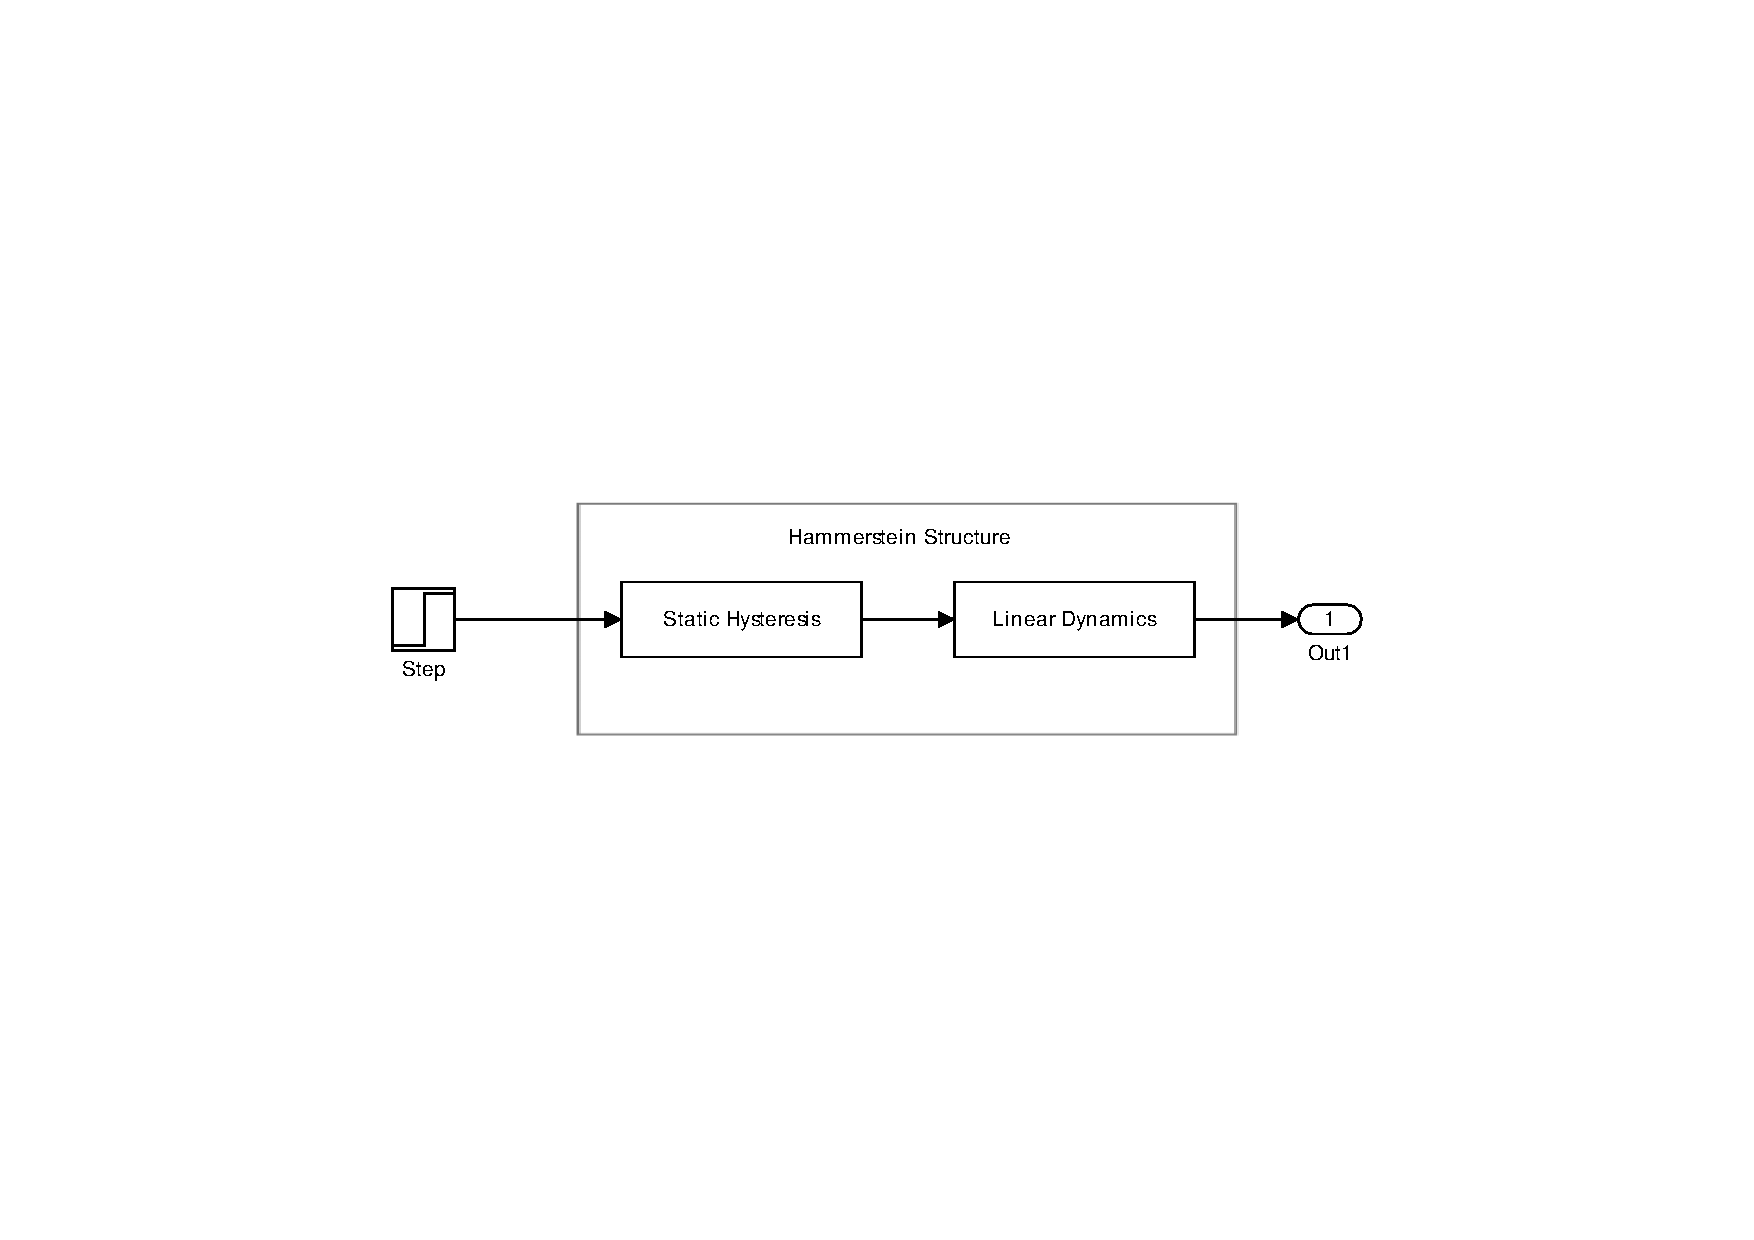
\includegraphics[width=0.7\textwidth, trim=8cm 8cm 7.73cm 8cm, clip=true]{fig/matlab/hammerstein}
  \caption{\label{fig:hammerstein}Block diagram of a Hammerstein structure, consisting of two blocks in series, modeling the static hysteresis and the linear dynamics, respectively.}
\end{figure}

\subsection{Maxwell-slip Model}
\label{sec:maxwell}
A generalized Maxwell-slip is used to model the hysteresis effect. It uses a parallel $n^{th}$ order elasto-slide element system with a friction force acting on each element, to create a nonlinear model. An elasto-slide element consist of a massless spring connected in series with a massless block that is subject to Coulomb friction. The inverse hysteresis model is summarized in the following equations and described more thoroughly in \citep{Ru:2016},

\begin{equation}
  \label{eq:maxwell_slip}
  F_i =
  \begin{cases}
    k_i(x - x_{bi}) & \quad \text{if }  k_i|x - x_{bi}| < f_i\\
    f_i\sgn(\dot{x}) \text{ where }  x = x_{bi} + \frac{f_i}{k_i}\sgn(\dot{x})  & \quad \text{else}\\
  \end{cases}
\end{equation}

\begin{equation}
  \label{eq:maxwell_sum}
  F = \displaystyle\sum_{i=1}^{n} F_i
\end{equation}

where $F_i$ is the output force, $k_i$ the spring constant, $f_i$ the break-away force and $x_b$ is the block position where $i=1 \hdots n$. In terms of the rotational stage $F_i$ represents the applied voltage, $x$ the input (rotational) displacement, $x_b$ angular position and $k_i, f_i$ are unknown parameters
The model parameters have been estimated by fitting the model to the major hysteresis loop, obtained by acquiring data from the system with a 0.5 Hz input driving signal as described in \citep{ButcherIdentification:2015,ButcherController:2015}. The identified set of parameters is presented in Table~\ref{tab:maxwell} where $n=10$. The model fit of the hysteresis model, which uses the same set of parameters as the inverse hysteresis model, is shown Figure~\ref{fig:maxwell}.

\begin{figure}[h]
  \centering
  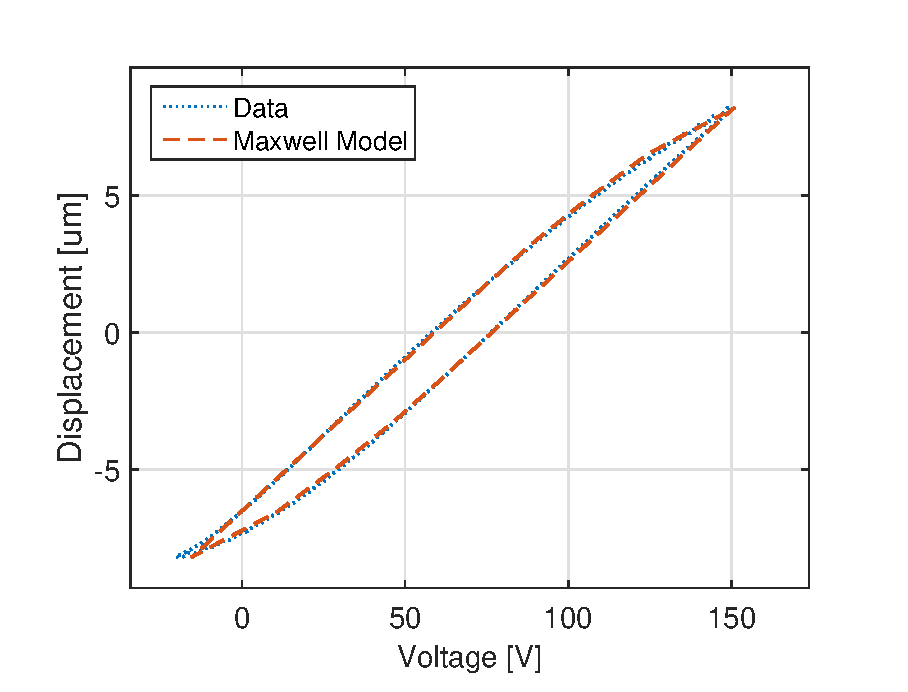
\includegraphics[width=0.7\textwidth]{fig/matlab/maxwell.eps}
  \caption{\label{fig:maxwell} Model fit of the Maxwell slip model to the acquired hysteresis of the rotational stage. The fit has a mean squared error of 1.1464.}
\end{figure}

\begin{table}[h!]
  \centering
  \begin{tabular}{| l | l | l |}
    \hline
    $i$ & $k_i$ & $f_i$ \\ \hline
    1 & 4.53 & 3.69 \\
    2 & 0.90 & 1.46 \\
    3 & 1.01 & 2.47 \\
    4 & 0.36 & 1.16 \\
    5 & $1.49 \times 10^{-6}$ & $4.28 \times 10^{-6}$ \\
    6 & $2.89 \times 10^{-7}$ & $1.41 \times 10^{-6}$ \\
    7 & $1.59 \times 10^{-7}$ & $9.10 \times 10^{-7}$ \\
    8 & $1.39 \times 10^{-7}$ & $9.10 \times 10^{-7}$ \\
    9 & $2.28 \times 10^{-7}$ & $1.67 \times 10^{-6}$ \\
    10 & $4.58$ & 37.30 \\
    \hline
  \end{tabular}
  \caption{\label{tab:maxwell} Identified parameters of the Maxwell slip model.}
\end{table}

\subsection{Linear System Identification}
\label{sec:linsys}
The extracted linear dynamics have been identified as a $6^{th}$ order transfer function using a \abbrPRBS as excitation signal, allowing for a valid extraction from the nonlinear dynamics. The system transfer function has been derived in discrete-time using the System Identification Toolbox in Matlab. A more detailed description of the procedure is available in \citep{ButcherController:2015}. The transfer function of the model (at 3.25 V), discretized with a sampling time of \unit{0.5}{\milli\second}, is presented in \eqref{eq:tf}.

\begin{equation}
  \label{eq:tf}
  G(z) = \frac{21.05z^{-1} - 6.85z^{-2} + 8.52z^{-3} - 0.71z^{-4} + 9.30z^{-5}}{1344 - 2481z^{-1} + 1469z^{-2} + 21.64z^{-3} - 1767z^{-4} + 2084z^{-5} - 639.5z^{-6}}
\end{equation}

The transfer function uses five zeros and and six poles to model two of the major resonances as seen in Figure~\ref{fig:model}, which shows a comparison between the model and the calculated Fast Fourier Transform (\abbrFFT) of the real system. The \abbrFFT was calculated by dividing the \abbrFFT of the output with the \abbrFFT of the input.

\begin{figure}[h!]
  \centering
  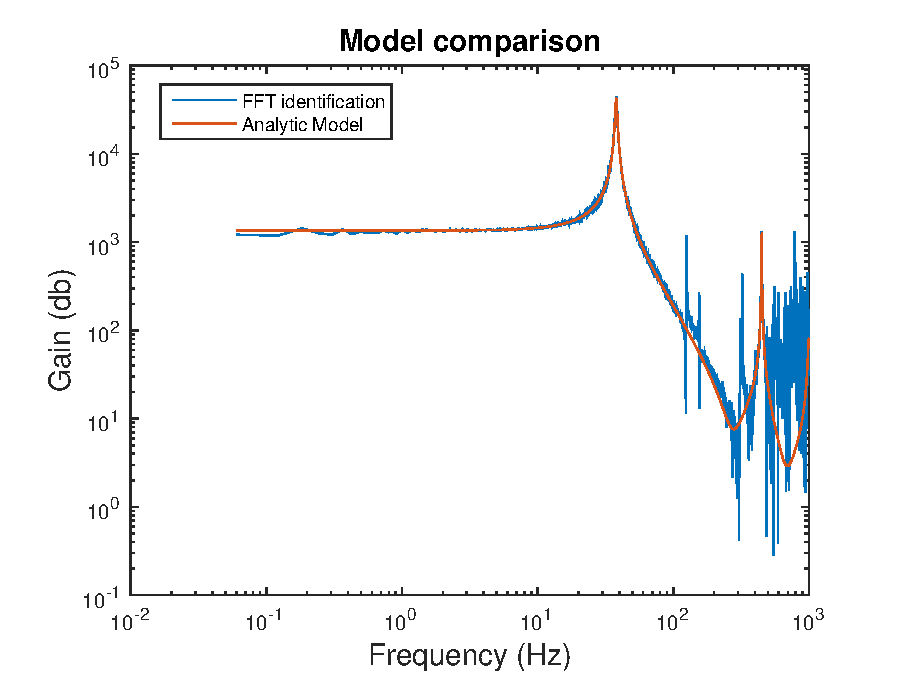
\includegraphics[width=0.7\textwidth]{fig/matlab/model.eps}
  \caption{\label{fig:model} Model fit of the system model with 5 zeros and 6 poles shown in \eqref{eq:tf} to the \abbrFFT of the acquired data.}
\end{figure}

\FloatBarrier
\section{Present Control Approach}\label{sec:presentControlApproach}
The original controller for the rotational stage is a 2-\abbrDOF structure (feedback and prefilter). A schematic overview of the control loop is depicted in Figure~\ref{fig:present}, consisting of a controller block C, a prefilter F, a disturbance d and the linearized rotational stage $G = H^{-1}G_0$, where $G_0 = HG$ contains both the nonlinear and linear dynamics and $H^{-1}$ is the hysteresis compensator.

\begin{figure}[h!]
  \centering %crop: left bottom right top
  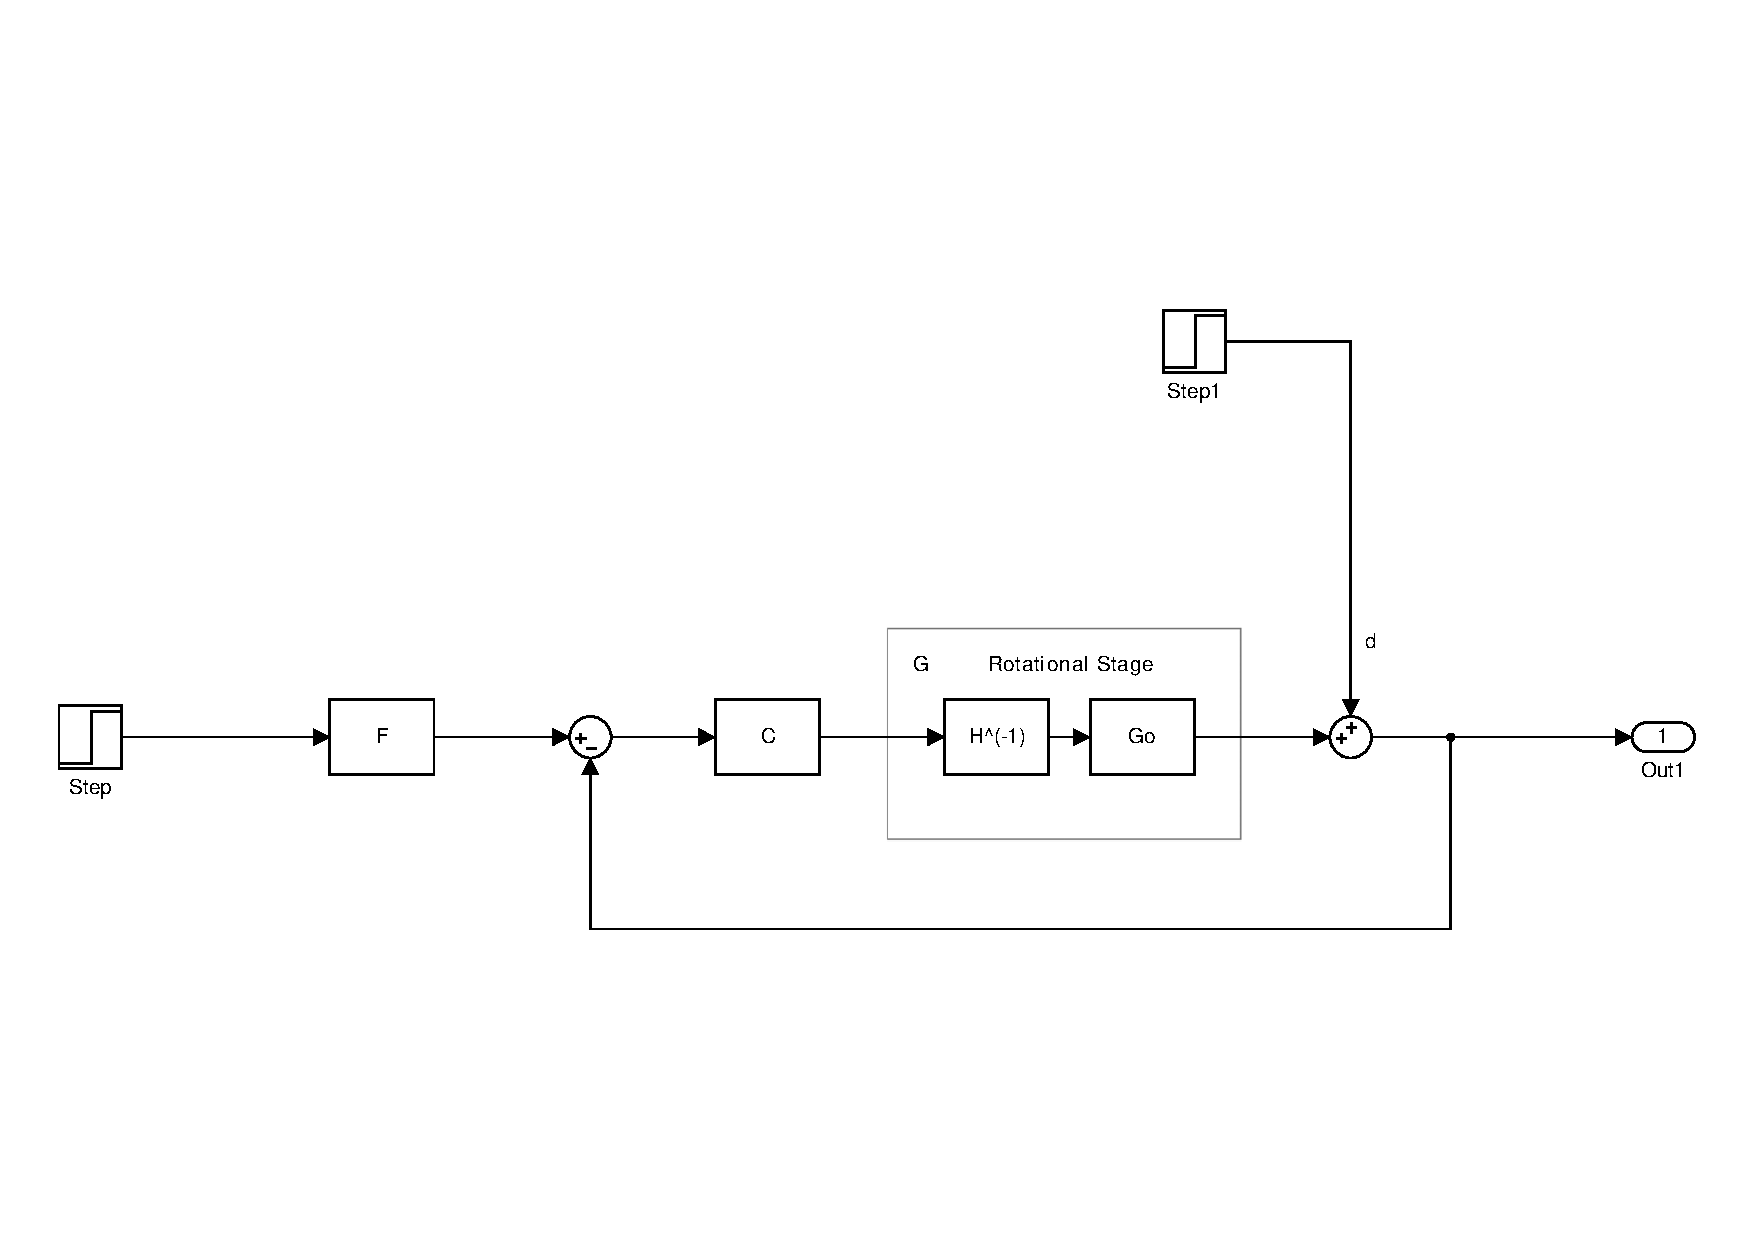
\includegraphics[width=0.95\textwidth, trim=4cm 4cm 2.1cm 10cm, clip=true]{fig/matlab/present_controller}
  \caption{\label{fig:present}Block diagram of the present control loop, including controller, prefilter and hysteresis compensator.}
\end{figure}

The controller block (C) is a series combination of a \abbrPID controller, a notch filter and a lead filter, which stabilizes the system (\abbrPID), increases the phase margin (lead) and makes the system more robust to high frequency oscillations (notch). Since the open loop bandwidth is relatively low, $f_b$ = 58 Hz according to Figure~\ref{fig:model}, it was decided to exclude cancellation of the first resonance peak in order to maintain the bandwidth as high as possible and to have sufficient attenuation of the first resonance peak \citep{ButcherController:2015}. Finally, to enhance the tracking performance, a prefilter (F) was also added to the system. The PID controller, lead network, notch filter and prefilter are all presented below in \eqref{eq:controller}.

\begin{subequations}
  \label{eq:controller}
\begin{alignat}{2}
  \label{eq:pre}
  & F(z) = \frac{0.0029z - 0.0029}{z^3 - 2.91z^2 + 2.816 z - 0.91} \\
  \label{eq:pid}
  & C_{PID}(z) = \frac{0.47z^2 - 0.94z + 0.47}{z^2 - 1.78 z + 0.78} \\
  \label{eq:lead}
  & C_{lead}(z) = \frac{4.20 z^2 - 7.72z + 3.55}{z^2 - 1.67z + 0.69} \\
  \label{eq:notch}
  & C_{notch}(z) = \frac{0.28z^4 - 0.62z^3 + 0.75z^2 - 0.59z + 0.26}{z^4 - 1.95z^3 + 1.39z^2 - 0.40z + 0.039}
\end{alignat}
\end{subequations}

The effect of each filter can be seen in Figure~\ref{fig:opensys}, where the open loop system is plotted with one filter added at a time. One can see that the high resonance peak is mitigated after the notch filter has been added, the lead filter rises the phase and that the \abbrPID controller provides good phase as well as good gain margin. Also the closed loop system is presented in Figure~\ref{fig:closedsys}, proving that the prefilter increases the closed loop bandwidth. The final closed loop bandwidth is 9.7 Hz.

\begin{figure}[h!]
  \centering %crop: left bottom right top
  \subfloat[][\label{fig:opensys} Open loop]{
  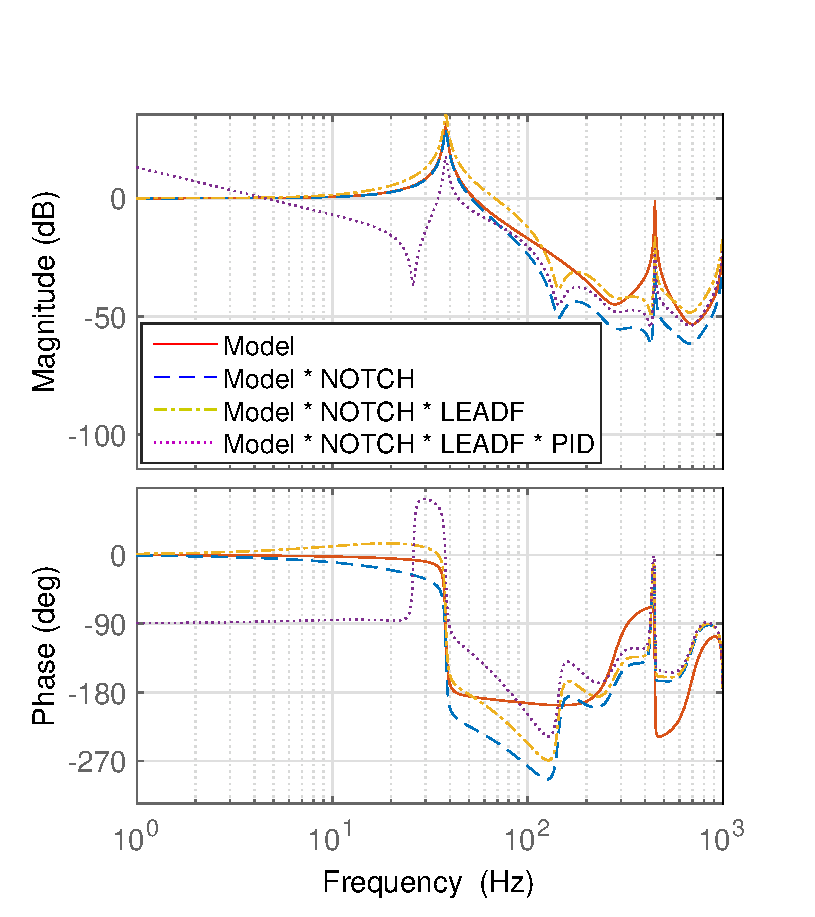
\includegraphics[width=0.46\textwidth, trim=0cm 0cm 1cm 0cm, clip=true]{fig/matlab/openloop_sys.eps}}
  \qquad
  \subfloat[][\label{fig:closedsys} Closed loop]{
  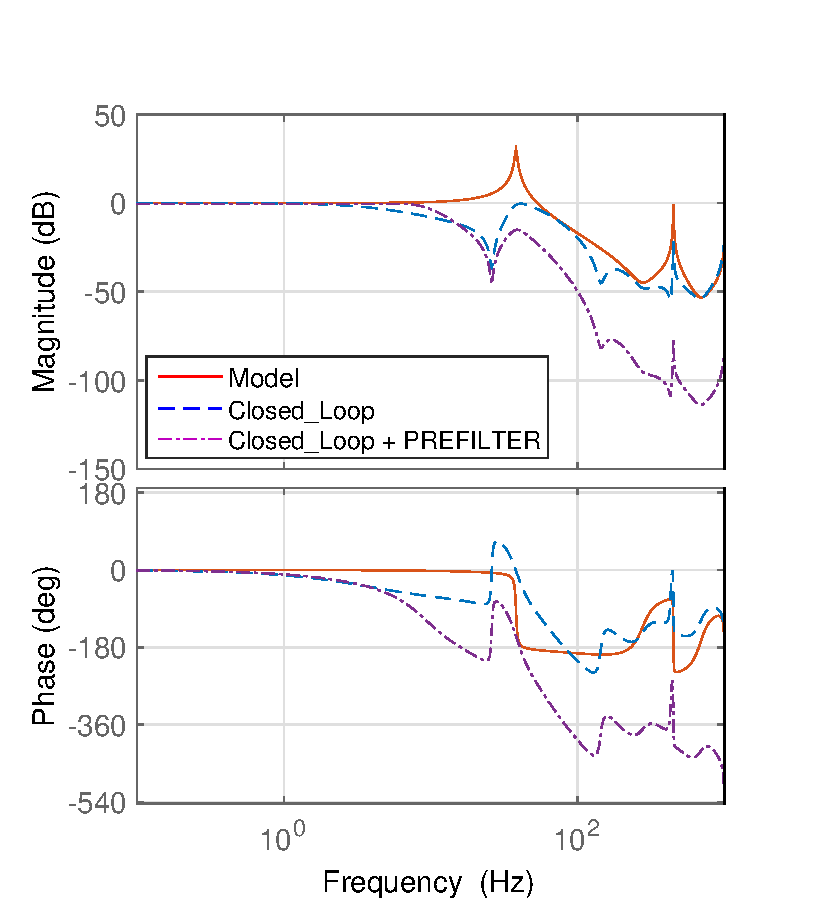
\includegraphics[width=0.46\textwidth, trim=0cm 0cm 1cm 0cm, clip=true]{fig/matlab/closedloop_sys.eps}}
  \caption{\label{fig:open_and_closed_sys} Illustration of controller effect. The effect of adding the different filters is shown in the open loop bode plot in (a) with the resulting closed loop system, with the open loop containing all filters, in (b). }
\end{figure}
